\documentclass{stsci_report}
\usepackage{deluxetable}
\usepackage{graphicx}
%\usepackage{amsmath}
%\usepackage{amsfonts}
\usepackage{latexsym}
%\usepackage{siunitx}
\usepackage{xcolor}
%\usepackage{times}

\bibliography{bibliography.bib}

\copyrighttext{Copyright\copyright\ \the\year\ The Association of Universities for Research in Astronomy, Inc. All Rights Reserved.}

\presubtitle{Instrument Science Report HST 2014}
\title{\textbf{Cycle 21-24 HST+COS\\Target Acquisition Monitoring}}
\author{Steven V. Penton}
\date{\today}

\DeclareGraphicsRule{.ps}{eps}{.ps}{}
\definecolor{green}{rgb}{0, 1.0, 0}
\definecolor{red}{rgb}{1,0,0}
\definecolor{blue}{rgb}{0,0,1}
\definecolor{Lblue}{rgb}{0.8,0.85,1}
\definecolor{darkgreen}{rgb}{0.25,1.0,0.25}
\definecolor{Brown}{cmyk}{0, 0.8, 1, 0.6}
\definecolor{Yellow}{rgb}{1, 1, 0}
\definecolor{Light}{gray}{.80}
\definecolor{Dark}{gray}{.20}

%\newcommand{\numpos}{{\bf NUM$\_$POS}\rm}
\newcommand{\psiafdate}{2010.060}
\def\arcsec{\hbox{$^{\prime\prime}$}}
\def\degree{\hbox{$^{\circ}$}}
\newcommand{\nokmsno}{{\rm km~s}\ensuremath{^{-1}}}
\newcommand{\kmsno}{~\nokmsno}
\newcommand{\kms}{~\nokmsno\ }
\newcommand{\tacq}[1]{\texttt{ACQ/#1}}

\begin{document}
\maketitle

\abstract{This ISR documents the HST+COS Target Acquisition (TA) monitoring programs for HST Cycles 21-24. During this period, FUV exposures were executed at Lifetime Positions (LP) LP2 and LP3, and all NUV exposures were obtained at the nominal (LP1) position.
These programs were designed to monitor numerous aspects of both imaging and spectroscopic COS TAs, including checking the TA subarrays, monitoring the required flashes of the internal PtNe lamps, and evaluating the accuracy of numerous COS flight software (FSW) patchable constants required for TA. This project verified that all three COS TA modes (FUV spectroscopic, NUV spectroscopic, and NUV imaging) were behaving nominally in Cycle 21-24, and determined that no SIAF or FSW parameter updates were required during this time.
There were, however, changed required for MIRRORB NUV \texttt{ACQ/IMAGE}s. These changes included a changing of the lamp current from LOW to MEDIUM, an adjustment of the \texttt{LTACAL} exposure time, and a modification of both the MIRRORB WCA and PSA/BOA  \texttt{ACQ/IMAGE} subarrays.
}

%\vspace{-0.3cm}
\section*{Contents}
%\vspace{-0.3cm}

\begin{itemize}
\item Introduction (page \pageref{sec:Introduction})
\item COS TA Operations Summary (page \pageref{sec:TAoperations})
\item Program Descriptions (page \pageref{sec:programs})
\item SIAF Verification (page \pageref{sec:siaf})
\item Imaging TA Verifiation (page \pageref{sec:NimVER})
\item Spectroscopic TA Verification (page \pageref{sec:spVER})
\item TA Subarray Verification (page \pageref{sec:subarray})
\item Results (page \pageref{sec:results})
\item Conclusion (page \pageref{sec:theend})
\end{itemize}
\clearpage
\section{Introduction}\label{sec:Introduction}

Preliminary results of the Hubble Space Telescopes' (HST) Cosmic Origins Spectrograph (COS) target acquisition (TA) programs reviewed here were previously reported in the following COS ISRs:
\small
\begin{itemize}
\item{COS ISR 2015-02 (Summary of the COS Cycle 20 Calibration Program)}
\item{COS ISR 2015-06 (Summary of the COS Cycle 21 Calibration Program)}
\item{COS ISR 2016-03 (Summary of the COS Cycle 22 Calibration Program)}
\item{COS ISR 2016-09 (Cycle 22 COS Target Acquisition Monitor Summary)}
\item{COS ISR 2017-18 (Cycle 23 COS Target Acquisition Monitor Summary)}
\item{COS ISR 2018-09 (Cycle 24 COS Target Acquisition Monitor Summary)}
\end{itemize}
\normalsize
The information in this ISR supercedes any previous preliminary results or conclusions.\\

This ISR provides the full details of the following HST+COS calibration {\bf P}rograms:
\small
\begin{itemize}
\item{P13124 (COS Imaging TA and Spectroscopic WCA-PSA/BOA offset verifications, Cycle 20)}
\item{P13526 (COS Imaging TA and Spectroscopic WCA-PSA/BOA offset verifications, Cycle 21)}
\item{P13972 (COS Imaging TA and Spectroscopic WCA-PSA/BOA offset verifications, Cycle 22)}
\item{P14440 (COS Imaging TA and Spectroscopic WCA-PSA/BOA offset verifications, Cycle 23)}
\item{P14857 (COS Imaging TA and Spectroscopic WCA-PSA/BOA offset verifications, Cycle 24)}
\end{itemize}
\normalsize

There are three modes of Target Acquisition (TA) for the Cosmic Origins Spectograph (COS); NUV imaging, NUV spectroscopic, and FUV spectroscopic.
There are four COS TA (\tacq{}) procedures; \tacq{IMAGE}, \tacq{PEAKD}, \tacq{PEAKXD}, and \tacq{SEARCH}. The \tacq{PEAKD} and \tacq{SEARCH}
step the telescope through dwell patterns on the sky. As long as the target light falls correctly within
the TA detector sub-arrays, \tacq{PEAKD} and \tacq{SEARCH} will continue to nominally assist in TA (barring any unforeseen anomalies). The \tacq{IMAGE} and \tacq{PEAKXD} procedures rely on the sub-arrays and patchable constants
in the COS flight software (FSW) which assist in target centering. In both \tacq{IMAGE} and \tacq{PEAKXD}, the internal
wavelength calibration lamp is flashed to locate the center of the wavelength calibration aperture (WCA). From this location, the center of the
science aperture (SA) in use, which could be the PSA or BOA, can be predicted by applying the FSW constant that give the SA offset compared to the WCA center. For \tacq{IMAGE},
the offset is in both detector `X' (along-dispersion, AD) and `Y' (cross-dispersion, XD). For \tacq{PEAKXD}, which uses dispersed light, this offset is only in the Y (XD) direction. All programs verify that the TA subarrays
in use for the given cycle were proper for the modes tested, and verifiies the actively used WCA-to-SA offsets to monitor the performance of COS TAs.

\tacq{IMAGE} has four combinations of two SAs, the Primary Science Aperture (PSA) and the Bright
Object Aperture (BOA), and two mirror modes, MIRRORA and MIRRORB. Each combination is commonly used, and has a slightly different WCA-to-SA offset in both X (AD) and Y(XD), which must be verified.

BOA spectroscopic TAs were not supported for COS during Cycles 20-14, so these programs only verify the PSA spectroscopic TAs.
WCA-to-PSA offsets are used in \tacq{PEAKXD}s, and each COS grating has a different WCA-to-SA XD offset. For each FUV lifetime position (LP),
the FUV gratings have different offsets. The programs listed here verify the NUV LP1 as well as the FUV LP2 and LP3\footnote{The COS FUV channel was moved to LP3 on February 15, 2015.} position offsets.
The FUV LP4 uses a different \tacq{PEAKXD} algorithm ({{\bf NUM$\_$POS}\rm}$>1$), and, like \tacq{PEAKD} does not use the WCA-to-SA XD offsets.

The CAS TA centering requirements are based upon the wavelength accuracy requirements in the AD, and for flux and resolution optimization
in the XD. The strictest NUV requirements are [AD,XD] = [0.041, 0.3]\arcsec, while for the FUV they are [AD,XD] = [0.106, 0.3]\arcsec. While the XD
requirement for all TAs center is $\pm$ 0.3\arcsec, our 1$\sigma$ goal is $\pm$ 0.1\arcsec.\footnote{This goal ensures that spectra fall on a consistent XD location on the the detector, which aids in extraction and calibration accuracy.}

In \S~\ref{subsec:acqimage} we will discuss the verification of the FSW parameters, lamp operations, and subarrays associated with COS \tacq{image}s.
As outlined in \S~\ref{subsec:fgs2si}, data from outside the COS calibration programs listed above will be used in this analysis.
As part of this process, we will verify the active COS NUV SIAF (Science Instrument Aperture File) entries. In ~\S~\ref{sec:spVER},
we will discuss the verification of the FSW parameters, lamp operations, and subarrays associated with COS spectroscopic TAs.
In the FUV sub-section we will discuss and the verification of COS FUV SIAF entries.

\subsection{Introductory Notes and Conventions}\label{sec:intro}
%\vspace{-0.3cm}
There are a few COS conventions to be established before discussing TA in detail.
\begin{enumerate}
	\item{COS TAs are performed in raw or ``detector'' coordinates, not the ``user'' coordinate system of calibrated
		COS files. To avoid confusion over the different coordinate systems, we will use along-dispersion (AD) and cross-dispersion (XD) whenever possible.
		All references to the coordinates ``X'' and ``Y'' are in the detector coordinate system unless otherwise specified.
		In raw NUV coordinates, +X is the +XD and +Y is -AD. In raw FUV coordinates, +X is -AD and +Y is +XD.
		The transformations between user and detector coordinates are :
		\begin{equation} NUV: X_{user} = 1023 - Y_{detector} \ ; Y_{user} = 1023-X_{detector} \end{equation}
		\begin{equation} FUV: X_{user} = 16383 - X_{detector} \ ; Y_{user} = Y_{detector} \end{equation}
		}
	\item{To emphasize the names of various TA parameters:
		\begin{itemize}
			\item{Keywords in FITS headers will be in \textit{ITALICIZED ALL CAPITALS}.}
			\item{COS TA modes and optional parameters will be in \texttt{Courier} (e.g., 	\tacq{IMAGE}).}
			\item{Parameters in the COS flight software (FSW) will be in \textsc{small capitals}.
In the FSW, all parameters begin with ``\textsc{pcta\_}''. In this TIR, this prefix is considered implied and is not included,
except in the tables and descriptions in the appendices.}
			\item{COS FITS filenames, or portions of a filename, will be in {\sf sans-serif}.}
		\end{itemize}
	}
	\item{There are three centering options during \tacq{SEARCH} and \tacq{PEAKD}. In the Astronomers Proposal Tool (APT), these are
		referred to as \texttt{CENTER}=\texttt{FLUX-WT}, \texttt{FLUX-WT-FLR}, and \texttt{BRIGHTEST}.
		These parameters have slightly different names in the IHB, the FITS keywords, and the FSW.
		In this ISR, we will refer to the centering options as \texttt{CENTER}=\texttt{Flux-Weighted(FW)}, \texttt{Flux-Weighted-Floor(FWF)}, and \texttt{Return-To-Brightest(RTB)}.
	}
	\item{When discussing the various subarrays used during COS TA, boxes will be specified by giving the lowest
		valued corner (C) and full size (S) for both X and Y. A box is fully specified by giving its XC, XS, YC, \& YS. In this TIR, these will always be given in detector coordinates.}
	\item{When referencing NUV pixels, we will abbreviate pixel as p. For the FUV, we use DE to reference the FUV digital elements.}
	\item{Milli-arcseconds (0.001\arcsec) will be abbreviated as mas. }
	\item{COS contains numerous FUV and NUV central wavelength settings, which are defined in the FSW by the OSM1 or OSM2 rotation positions.
	In this ISR, the term CENWAVE will be used to mean any of the pre-defined OSM1 + OSM2 rotation settings that uniquely define a central wavelength setting.}
	\item{COS CENWAVEs are named for the (predicted) lowest wavelength that lands on the FUVA detector segment for FP-POS=3. For convienence, when referring to
	a specific CENWAVE will call out the grating and CENWAVE is use as GRATING/CENWAVE (e.g. G130M/1222). For convienence, we will occasionally use just a leading "C" to identify
	a particular CENWAVE (e.g., C1222) in the same manor as "G" is used for GRATING (e.g., G130M).}
	\item{When referring to an HST program number, we will use either "HST PID" or just a leading "P" in a similar fashion an "C=CENWAVE" and "G=GRATING".}
	\item{The COS FUV detector has two independent segments, Segment-A and Segment-B. In this ISR, they will be referred to as FUVA and FUVB.}
	\item{When referring to a particular day, we will use YEAR.DAY. For example, day 60 of 2010 will be referred to as \psiafdate. We will also occasionally use decimal years. In these cases, there will only be a single digit in the fractional part (e.g., 2009.9).}
	\item{Archived COS files are in FITS format (.fits) and the filenames are in the form {\sf IPPPSSOOT\_{\it extension}.fits}.
The HST naming convention breaks down for COS as I=Instrument=``L'', PPP=Program ID, SS=Visit ID, OO=Exposure ID,
and T=``Q'' for nominally recorded observations. See the COS DHB for a full breakdown of the HST IPPPSSOOT naming conventions.
COS TA files have the {\it extension} of {\sf rawacq}, and additional
TA information is contained in the {\sf IPPPSSOOT\_{\it spt}.fits} file known as the support file.}
\end{enumerate}

\section{COS TA Operations Summary}\label{sec:TAoperations}
There are 3 modes of COS target acquisition (TA); NUV imaging, NUV and FUV spectroscopic.
There are 4 COS TA (\tacq{}) procedures; \tacq{SEARCH}, \tacq{IMAGE}, \tacq{PEAKD}, and \tacq{PEAKXD}. \tacq{PEAKD}~ and \tacq{SEARCH}~ step the telescope through dwell patterns on the sky. As long as the target light falls completely within
the TA detector subarrays, \tacq{PEAKD}~ and \tacq{SEARCH}~ will continue to operate nominally.
In addition to proper TA subarrays, \tacq{IMAGE}, and \tacq{PEAKXD} \footnote{At FUV LP3, all \tacq{PEAKXD}~observations use the optional parameter {{\bf NUM$\_$POS}\rm}=1.} require accurate TA-associated flight software (FSW) patchable constants.
P14857 verifies that all Cycle~24 NUV and FUV TA subarrays are proper, and evaluates if the actively used WCA-to-PSA offsets\footnote{No BOA spectroscopic TAs were performed in Cycle~24, so these offsets were not verified.} are correct.
The initial HST/COS target pointing is based on definitions of the physical locations of the COS apertures in terms of [V2,V3] in the Science Instrument Aperture File (SIAF).
All of the actively used NUV (LP1) and FUV (LP3\footnote{The default COS FUV spectral location was moved to LP3 on February 15, 2015, for all central wavelength settings except G130M/1055 and G130M/1096, which still operate at LP2. On October 2, 2017, the default location of COS FUV spectra were moved to LP4, with additional observing and TA constraints as outlined on the COS2025 website (http://www.stsci.edu/hst/cos/cos2025).}) SIAF entries used for TA are also verified in this program.

In both \tacq{IMAGE}~ and \tacq{PEAKXD}\footnote{Beginning in Cycle~25, the \tacq{PEAKXD}~algorithm was enhanced so that two distinct algorithms can be employed.
The original \tacq{PEAKXD}, used in Cycles 19-24, is referred to as {{\bf NUM$\_$POS}\rm}=1, while the Cycle~25 (LP4) algorithm
uses the \tacq{PEAKD}~algorithm, but in the cross-dispersion (XD) direction and is referred to as the {{\bf NUM$\_$POS}\rm}~$>1$ \tacq{PEAKXD}.},
 the internal wavelength calibration lamp is flashed to locate the wavelength calibration aperture (WCA). From its measured location on the detector, the center of the science aperture (SA) in use can be predicted by applying the FSW constants that give the SA offset compared to the WCA center for the combination of optics in use.
For \tacq{IMAGE}, the offset is in both the along-dispersion (AD) and cross-dispersion (XD) directions. For \tacq{PEAKXD}, which uses dispersed light, this offset is only in the XD direction.
\begin{itemize}
\item{The \tacq{IMAGE}~procedure has four combinations of two SAs, the Primary Science Aperture (PSA) and the Bright Object Aperture (BOA), and two mirror modes, MIRRORA and MIRRORB. Each combination is commonly used, and has a different WCA-to-SA offset in both AD and XD, which must be verified\footnote{These offsets are maintained in the FSW as the patchable constant tables \textsc{pcta\_ImCalTargetOffset} (XD) and \textsc\textsc{pcta\_YImCalTargetOffset} (AD).}. \tacq{IMAGE}s~also rely on accurate AD and XD plate scales. These physical plate scales should remain constant for the NUV MAMA and are not monitored or tested by this program.
}
\item{The \tacq{PEAKXD}~procedure used in Cycle~24 relies upon FSW XD WCA-to-PSA offsets\footnote{Maintained in the FSW patchable constant table \textsc{pcta\_CalTargetOffset} for both NUV and FUV.}, and grating-specific XD plate scales\footnote{Maintained in the FSW patchable constant tables \textsc{pcta\_NUVMilliArcsecsPerPixelXDisp} and \textsc{pcta\_FUVMilliArcsecsPerPixelXDisp}.}
Each COS grating, SA, and lifetime position (LP) combination has a different offset. This program verifies all 4 NUV LP1 and 3 FUV LP3 grating-specific WCA-to-PSA offsets but does not test or monitor the FSW XD plate scales.
}
\item{This program does not attempt to monitor the AD accuracy of the COS spectroscopic TA modes.\footnote{For \tacq{PEAKD}, short-term fluctuations of the detector background rate due to environmental conditions remains the largest source of along-dispersion pointing error.}
}
\end{itemize}

COS centering requirements are based on wavelength accuracy in the AD, and flux and resolution in the XD. The strictest NUV requirements are [AD,XD] = [0.041, 0.300]\arcsec. For the FUV channel, they are [AD,XD] = [0.106, 0.300]\arcsec. The XD requirement for all TAs is centering to within $\pm$ 0.3\arcsec\ with a 1$\sigma$ goal of $\pm$ 0.1\arcsec.

\subsection{COS TA Centering Requirements}\label{subsec:requirements}

For COS TA, we take the CEI spec (0.3\arcsec) to refer to the required centering accuracy in the XD, and the wavelength requirements to apply to
the TA accuracy required in the AD direction. Since the AD requirement is in units of \kmsno, it is detector and wavelength
dependent as defined in equations~\ref{eq:TAcenter}--\ref{eq:TAcenterL}.
Assuming that the wavelength error budget is split evenly between the COS TA and wavelength scale accuracies,
the error budgets for the COS gratings, in arc-seconds (\arcsec), are given in Table~\ref{tab:TAaccuracy}. By ``evenly'' we mean that when added in quadrature the total error budget is that given by the second column of Table~\ref{tab:TAaccuracy}.
Setting the TA error budget equal to the wavelength scale accuracy, the AD TA requirement given in the third column is the second column divided by $\sqrt{2}$.
\small
\begin{eqnarray}\label{eq:TAcenter}
\Delta\ AD(G185M@1825\AA) = {{ 15\kms \times 1825\AA}\over{c \times 0 .037\AA/p\times 42.47 p/\arcsec}}  = 0.058\arcsec\\
\Delta\ AD(G225M@2250\AA) = {{ 15\kms \times 2250\AA}\over{c \times  0.035\AA/p\times 42.47 p/\arcsec}}  = 0.076\arcsec\\
\Delta\ AD(G285M@2850\AA) = {{ 15\kms \times 2850\AA}\over{c \times  0.040\AA/p\times 42.47 p/\arcsec}}  = 0.084\arcsec\\
\Delta\ AD(G230L@2450\AA) = {{175\kms \times 2450\AA}\over{c \times  0.390\AA/p\times 42.47 p/\arcsec}}  = 0.086\arcsec\\
\Delta\ AD(G130M@1300\AA) = {{ 15\kms \times 1300\AA}\over{c \times 0.00997\AA/ p\times 43.5 p/\arcsec}} = 0.150\arcsec\\
\Delta\ AD(G160M@1600\AA) = {{ 15\kms \times 1600\AA}\over{c \times 0.01223\AA/ p\times 42.9 p/\arcsec}} = 0.153\arcsec\\
\Delta\ AD(G140L@1800\AA) = {{150\kms \times 1800\AA}\over{c \times 0.08030\AA/ p\times 45.4 p/\arcsec}} = 0.247\arcsec\label{eq:TAcenterL}
\end{eqnarray}
\normalsize
\clearpage

\begin{deluxetable}{|c||c|c|}
\tablewidth{0pt}
\tabcolsep 18pt
\tablecolumns{3}
\tablecaption{COS Along-Dispersion (AD) Centering Requirements.\label{tab:TAaccuracy}}
\tablehead{	\colhead{COS Grating} &
			\colhead{Total Error Budget} &
			\colhead{AD TA Requirement}
}
\startdata
G185M & 0.058\arcsec\ & 0.041\arcsec\\
G225M & 0.076\arcsec\ & 0.054\arcsec\\
G285M & 0.084\arcsec\ & 0.059\arcsec\\
G230L & 0.086\arcsec\ & 0.061\arcsec\\
\hline
G130M & 0.150\arcsec\ & 0.106\arcsec\\
G160M & 0.153\arcsec\ & 0.108\arcsec\\
G140L & 0.247\arcsec\ & 0.175\arcsec\\
\enddata
\tablecomments{Assuming the total error budget (column 2) is split equally between TA AD centering and wavelength scale accuracy,
the AD TA requirements (column 3) are 1/$\sqrt{2}$ of the total error budget (equations~\ref{eq:TAcenter}--\ref{eq:TAcenterL}).}
\end{deluxetable}


\section{Program Descriptions \label{sec:programs} }

In addition to COS calibration programs listed above, COS exposures obtained in numerous cycles of the "Focal Plane Calibration (SI-FGS Alignment)" series were used  in this ISR.
These programs were developed by the HST Telescope's division (PI Cox or ????) for Fine Guidance Sensor (FGS) to Science Instrument (SI) alignment, and are described in \S~\ref{subsec:fgs2si}

This program builds upon the monitoring and calibration of the FGS-to-SI alignment program (P14452 - HST Cycle 23- Focal Plane Calibration (SI-FGS Alignment)).  P14452 performs back-to-back PSA/MIRRORA and PSA/MIRRORB \tacq{IMAGE}s, from which all the results herein are bootstrapped.

All data with a given program/cycle were intentionally taken contemporaneously to avoid any long-term detector or spacecraft effects from affecting our results.
Our requirement was that all data for a given program were taken within 60 days of each other.\\

\subsection{FGS-to-SI Programs}\label{subsec:fgs2si}

From Cycles 17-23, an FGS-to-SI program executed with COS visits twice a year. These programs contained COS exposures designed to assist in the monitoring of the COS NUV alignent to HST.
These programs used the same two stars with COS in visits spaced six months apart. Both visits observed the astrometric open cluster M35, at orientations that were 180\degree~apart.
The two stars observed were 206W3 (in the Fall) and 427W3 (in the Spring). Due to time constraints, the exact content of the COS visits in these programs varied from year to year.

However, the COS portion of each program begins with a PSA+MIRRORA \tacq{IMAGE} on a target should be approximately centered due to observations with other instruments earlier in the Visit.
Post-observation telemetry data, an the results of the \tacq{IMAGE}, are used to refine this assumption.
This process verifies the COS NUV PSA aperture position\footnote{Specifically, the \textit{LFPSAA} entry.} in the SIAF to about 0.5 pixels or (~0.012\arcsec).

After this PSA+MIRRORA \tacq{IMAGE}, a PSA+MIRRORB \tacq{IMAGE} is then performed (a ``set'').
This bootstraps the PSA+MIRRORB centering to the PSA+MIRRORA and to the SIAF verification.
This allows us to monitor the properties of the PSA+MIRRORB image in a controlled way on a centered target.
Where possible, time-tag (\textbf{TT}) images of the lamps and/or targets along with NUV G230L

The historical list of FGS-to-SI proposals, cycles (C), and content were:
\begin{itemize}
	\item{11878 (Cycle~17):}{Two sets of PSA \tacq{IMAGE}s, Target+Lamp Time-Tag images, \& G230L Spectra}
	\item{12399 (Cycle~18):}{Two sets of PSA \tacq{IMAGE}s, One set of Target+Lamp Time-Tag images (427W3), one G230L Spectrum (427W3)}
	\item{12781 (Cycle~19):}{Two sets of PSA \tacq{IMAGE}s}
	\item{13171 (Cycle~20):}{Two sets of PSA \tacq{IMAGE}s}
	\item{13616 (Cycle~21):}{Two sets of PSA \tacq{IMAGE}s}
	\item{14035 (Cycle~22):}{Two sets of PSA \tacq{IMAGE}s}
	\item{14452 (Cycle~23):}{Two sets of PSA \tacq{IMAGE}s,  with Lamp-Only Time-Tag images after each \tacq{IMAGE}}
\end{itemize}

This verifies the COS NUV PSA aperture position in the SIAF. After this PSA+MIRRORA \tacq{IMAGE}, a PSA+MIRRORB \tacq{IMAGE} is then performed.
This exposure bootstraps the PSA+MIRRORB centering to the PSA+MIRRORA SIAF verification.
This allows us to monitor the properties of the PSA+MIRRORB image in a controlled way on a centered target.
No spectra are taken in P14452 due to time constraints, but we are currently planning on adding in PSA/MIRRORA and PSA/MIRRORB lamp images.

\subsection{COS TA Monitoring Program History}\label{subsec:History}
In the 2009 (STS-125) servicing mision orbital verification (SMOV) phase, a series of programs in NUV imaging mode carefully determined the two-dimensional offset from the WCA to the center of the PSA when observed with MIRRORA.
These X and Y offsets were loaded in the FSW parameters \textsc{pcta\_XImCalTargetOffset} and \textsc{pcta\_YImCalTargetOffset}.
A target was then centered using a PSA+MIRRORA \tacq{IMAGE}, then a target image was taken along with a MIRRORB image
of the WCA image. These images were used to determine the X and Y offsets of the image target and WCA centroids.
These values were uploaded in the FSW paramaters. This bootstrapping procedure was repeated with the BOA+MIRRORA
and BOA+MIRRORB \tacq{IMAGE} modes until all four \tacq{IMAGE} modes were co-aligned.

In this program (13972) we use this bootstrapping strategy to test the co-alignment of all four \tacq{IMAGE} modes.\footnote{On November 6, 2014,
the MIRRORB \tacq{IMAGE} wavelength calibration lamp exposure was changed from a 30 second exposure
at LOW current (3mA) to a 12 second exposure at MEDIUM current. At this point the \textsc{pcta\_XImCalTargetOffset} and \textsc{pcta\_YImCalTargetOffset}
FSW parameters were also updated to reflect a small change in the WCA-to-SA imaging MIRRORB offsets. This program is the first
to monitor the updated offsets.}
To accomplish this in only two orbits, this project leverages observations taken in FGS-to-SI alignment verification program (14035).

The FGS-to-SI program (P14035) performs a PSA/MIRRORA \tacq{IMAGE} on a target that should be centered in the aperture.
The PSA+MIRRORA \tacq{IMAGE} in Visit `A2' of P14035 can be used to verify the COS NUV PSA aperture position in the SIAF.
This exposure shows that the COS NUV PSA SIAF entry combined with the PSA+MIRRORA WCA-to-PSA offsets are
accurate to within [AD,XD] = [-0.020,0.105]\arcsec\ (this is the distance that the \tacq{IMAGE} slewed to center the target).
The COS aperture is only repeatable in the XD direction to $\pm$ one motor step (0.05\arcsec). In addition, the WCA location
cannot be measured to better than 1/2 pixel as the pixel used to determine the median location in an integer.
On the NUV detector, 1 pixel is $\sim$ 0.023\arcsec. Based upon this information, the COS NUV PSA definition
in the SIAF file appears to meet our accuracy requirements for Cycle 22.

After the P14035 Visit `A2' PSA+MIRRORA \tacq{IMAGE}, a PSA+MIRRORB \tacq{IMAGE} is performed.
This exposure bootstraps the PSA+MIRRORB centering to the PSA+MIRRORA + SIAF verification.
This allows us to monitor the properties of the PSA+MIRRORB image in a controlled way on a centered target. No spectra or images are taken in P14035 due to time constraints.
Visits 01 and 02 of P13972 extend the COS SIAF/FGS-to-SI verification of Visit 02 of P14035 to the other two \tacq{IMAGE} combinations (BOA+MIRRORA and BOA+MIRRORB) by bootstraping from the PSA+MIRRORB verification to co-align all the COS TA imaging modes. The details of the observations are given is the observing section.
Visit 01 of P13972 bootstraps off Visit 02 of P14035 to co-align the PSA+MIRRORB \tacq{IMAGE} mode to the BOA+MIRRORA. Visit 01 of P13972 executed within 45 days of Visit 02 of P14035, to ensure that no long term instrument or telescope focus changes impact our results.
Visit 02 of P13972 follows the style of Visit 01, and bootstraps from the BOA+MIRRORA mode to the BOA+MIRRORB TA imaging mode. Visit 02 should also occur within 45 days of visit 02 of P14035 and within 45 days of Visit 01 of P13972.
\clearpage

\subsection{COS TA Monitoring Program Structure}\label{subsec:structure}

In its generic format, each cycles TA monitoring program contains three single-orbit visits. The number of visits is mandated by the bootstrapping technique between the four different \tacq{IMAGE} SA+MIRROR combinations.

Each visit begins with a comparison of the centering of two \tacq{IMAGE}~modes out of the possible four science apertures (SA, PSA or BOA) $\times$ (MIRRORA or MIRRORRB).
This back-to-back \tacq{IMAGE}~ process allows us to test that all \tacq{IMAGE} modes are centering the target to the same point in the aperture.
Each of science aperture (SA) and MIRRORA/B ACO/IMAGE combinations were co-aligned during SMOV\footnote{The underlying assumption of these programs is that that the PSA/MIRRORA \tacq{IMAGE}~centering has not changed since SMOV.},
and rely on the flight software (FSW) WCA-to-SA along-dispersion (AD) and cross-dispersion (XD)
offsets\footnote{In the FSW, these parameters are stored in the \textsc{pcta\_XImCalTargetOffset} (XD) and \textsc{pcta\_YImCalTargetOffset} (AD).}.
This comparison involves not only the \tacq{IMAGE}s, but NUV detector images of the WCA lamp image and, if possible, coeval target images.
These direct lamp+target comparisons are only available for the PSA modes. For the BOA modes, the WCA lamp images and target images are taken consecutively.
The Lamp+target exposures are interleaved throughout the visit to measure and verify the imaging WCA-to-SA offsets are still accurate for each HST Cycle.
Images will usually use the PtNe\#2 (P2) lamp, as it is the primary TA lamp, but some images will use PtNe\#1 (P1) to monitor both lamps in imaging mode.

In its generic format, the three visits are configured as follows:
\begin{itemize}
	\item{The first orbit on this program is designed to test the co-alignment of the PSA+MIRRORA and PSA+MIRRORB \tacq{IMAGE} combinations.
However, this exact combination occurs at the end of each the semi-annual visits of the FGS-to-SI alignment program operated by the HST Telescopes' group.
This visit was usually treated as an on-hold contingency visit in case, for whatever reason, the fall visit of the program did not execute in a given cycle.\footnote{Beginning with Cycle 23, this program
was replaced with an improved process for aligning the FGSs so we needed to activate this visit to obtain the PSA/MIRRORA to PSA/MIRRORB \tacq{IMAGE}~ alignment.}
As discussed further in \S~\ref{sec:newMIRRORB}, in one case, Cycle 22XX (P1YYYY), this visit wos re-purposed to verify a change to the MIRRORB
\tacq{IMAGE} configuration required due to the increasing background.}
	\item{The second visit of this program takes back-to-back PSA/MIRRORB and BOA/MIRRORA \tacq{IMAGE}s~and target TIME-TAG images (with lamp flashes) and takes NUV and FUV spectra to test their WCA-to-PSA offsets.}
	\item{The third visit of this program takes back-to-back BOA/MIRRORA and BOA/MIRRORBA \tacq{IMAGE}s~and target TIME-TAG images (with lamp flashes) and takes NUV and FUV spectra to test test WCA-to-PSA offsets for gratings not tested in the second visit.}
\end{itemize}
The exact configuration of which gratings and which CENWAVEs were spectroscopically tested varied with each cycle as the programs evolved.
Specifically, with the change in OSM2 Home position, NUV spectra were re-ordered for efficiency and some NUV cenwaves were changed to those
that are known to have strong stripe B WCA spectra against the increasing detector background and declining NUV sensitivity.
In cycles 23 and 24, we took G160M/1600 exposures offset by {\bf POS$\_$TARG}s by +/- 0.7" to test for the effects of Ywalk on FUV spectra at LP3.
In addition, one visit of each program, usually the second visit, performed an annual a "family portrait"  of all the P1/P2 MIRRORA/B WCA lamp images to track any drifting of the centroids, or changes in the lamps with time.
Further details on the differences between the programs is provided in \S~\ref{subsec:differences}.

\subsection{Differences between TA monitoring programs}\label{subsec:differences}

There are several important differences between the various versions of the COS TA monitoring programs:

In the Cycle~21 HST+COS monitoring program,  \dots
In the Cycle~22 HST+COS monitoring program,  \dots
In the Cycle~23 HST+COS monitoring program,  \dots
In the Cycle~24 HST+COS monitoring program,  \dots
In the Cycle~25 HST+COS monitoring program, the visit names were changed from `01', `02', and `03' to `BA', `BB' , and `PB' to indicate which \tacq{IMAGE} mode was being tested; PB = PSA/MIRRORB, BA = BOA/MIRRORA, and BB = BOA/MIRRORB. Visits `BA' and `BB' of the Cycle~24 program are identical to Visits `01' and `02' of the Cycle~23 program in all other regards.
Visit `PB' of the Cycle~24 program is noticeably different than the contingency visit `03' in Cycle~23 program. The `PB' visit only includes those exposures absolutely required to compare the \tacq{IMAGE}~accuracy of PSA/MIRRORA to PSA/MIRRORB, while the Cycle~23 program also obtained spectra of all three FUV gratings for additional monitoring of spectroscopic TA performance under the assumption that detector `Y-walk' monitoring would benefit from additional observations near the end of the FUV LP3 lifetime. As all three visits of 14857 executed near the end of the LP3 lifetime, these additional exposures were not required.
The Cycle~24 version of the FGS-to-SI program was replaced with a better program (HST PID 14867\footnote{HST Cycle 24 Focal Plane Calibration (SI-FGS alignment), PI = Edmund Nelan.} for aligning the FGSs which did not allow the inclusion of these \tacq{IMAGE}~exposures\footnote{The FGSs were used as the prime science instrument in this proposal, which precluded the use of COS during the visit as COS is not an allowed parallel HST instrument.}.
For Cycle~24, we activated this visit to obtain the needed PSA/MIRRORA to PSA/MIRRORB \tacq{IMAGE}~alignment verification.

\clearpage

\subsection{Exposure Lists}\label{subsec:elists}

In Visit 01, we take spectra that meet these requirements with the G130M/1309, G140L/1280, G285M/2676, and G230L/3000, and in Visit 02,
we take spectra with the G160M/1600, G185M/1913, G225M/2306. Table ~\ref{tab:peakxd} the results of these exposures are summarized.
The rightmost column gives the WCA-to-PSA offsets measured in P13972, in arcseconds (\arcsec).
All exposures, except {\bf lcri01h6q}, the G140L/1280 measurement, which showed an offset of 0.15\arcsec\ exceed our $\pm 0.1$\arcsec\ goal.
All exposures exceed our $\pm 0.33$\arcsec\ requirement. The XD profile of G140L spectra is wider that the medium
resolution gratings (G130M and G160M), making in more susceptible to detector `Y-walk' (Penton \& Keyes, 2010).
No action is required at this time as the measured offset is 1/2 of our 0.3\arcsec\ requirement.

The final two exposures of the 02 visit intentionally offset the target by $\pm$ 0.7\arcsec\ to test the effects
of `Y-walk' on G160M \tacq{PEAKXD}s. All three G160M exposures in Visit 02 show offsets from the expected position
of $\le 0.05$\arcsec\ within our 0.1\arcsec\ goal. No action (e.g., updating the \textsc{pcta\_CalTargetOffset} in the FSW)
is required at this time.
%\startlongtable
\begin{deluxetable}{rrrrrrrrrrrrr}
\tabcolsep 2pt
\tabletypesize{\tiny}
\tablecolumns{13}
%\tablewidth{0 pt}
\tablecaption{COS/NUV TA Monitoring Imaging Exposures\label{tab:NUVtamonimage}}
\tablehead{
\colhead{ROOTNAME}&\colhead{PROP}&\colhead{TARGNAME}&\colhead{OBS} &\colhead{EXP}   &\colhead{EXP}  &\colhead{PtNe}&\colhead{Lamp}   &\colhead{APERTURE}&\colhead{APERXPOS}&\colhead{APERYPOS}&\colhead{OPT\_}&\colhead{DATE}\\
\colhead{}        &\colhead{ID}  &\colhead{}        &\colhead{MODE}&\colhead{TYPE}&\colhead{TIME(s)}&\colhead{Lamp}&\colhead{Current}&\colhead{}&\colhead{}&\colhead{ }&\colhead{ELEM}&\colhead{OBS}
}
\startdata
\hline
lc6ka1i1q	&	13171	&	427W3	&	ACCUM	&	ACQ/IMAGE	&	60	&	P2	&	Low	&	PSA	&	22.1	&	127.1	&	MIRRORA	&	2013-03-02	\\
lc6ka1i3q	&	13171	&	427W3	&	ACCUM	&	ACQ/IMAGE	&	300	&	P2	&	Low	&	PSA	&	22.1	&	127.1	&	MIRRORB	&	2013-03-02	\\
lc6ka2imq	&	13171	&	206W3	&	ACCUM	&	ACQ/IMAGE	&	60	&	P2	&	Low	&	PSA	&	22.1	&	127.1	&	MIRRORA	&	2013-09-01	\\
lc6ka2ioq	&	13171	&	206W3	&	ACCUM	&	ACQ/IMAGE	&	300	&	P2	&	Low	&	PSA	&	22.1	&	127.1	&	MIRRORB	&	2013-09-01	\\
lcgp01bpq	&	13523	&	WAVE	&	TT	&	WAVECAL	&	40	&	P2	&	Low	&	WCA	&	22.1	&	127.1	&	MIRRORB	&	2013-11-11	\\
lcgp01bsq	&	13523	&	WAVE	&	TT	&	WAVECAL	&	40	&	P1	&	Low	&	WCA	&	22.1	&	127.1	&	MIRRORB	&	2013-11-11	\\
lcgp01byq	&	13523	&	WAVE	&	TT	&	WAVECAL	&	20	&	P2	&	Low	&	WCA	&	22.1	&	127.1	&	MIRRORA	&	2013-11-11	\\
lcgp01c3q	&	13523	&	WAVE	&	TT	&	WAVECAL	&	20	&	P1	&	Low	&	WCA	&	22.1	&	127.1	&	MIRRORA	&	2013-11-11	\\
lci4a1dcq	&	13616	&	427W3	&	ACCUM	&	ACQ/IMAGE	&	60	&	P2	&	Low	&	PSA	&	22.1	&	127.1	&	MIRRORA	&	2014-04-03	\\
lci4a1deq	&	13616	&	427W3	&	ACCUM	&	ACQ/IMAGE	&	300	&	P2	&	Low	&	PSA	&	22.1	&	127.1	&	MIRRORB	&	2014-04-03	\\
lci4a2e3q	&	13616	&	206W3	&	ACCUM	&	ACQ/IMAGE	&	60	&	P2	&	Low	&	PSA	&	22.1	&	127.1	&	MIRRORA	&	2014-10-27	\\
lci4a2e5q	&	13616	&	206W3	&	ACCUM	&	ACQ/IMAGE	&	300	&	P2	&	Med	&	PSA	&	22.1	&	127.1	&	MIRRORB	&	2014-10-27	\\
lcgq01q5q	&	13526	&	WD-1657+343	&	ACCUM	&	ACQ/IMAGE	&	12	&	P2	&	Med	&	PSA	&	22.1	&	127.1	&	MIRRORB	&	2014-11-19	\\
lcgq01q7q	&	13526	&	WD-1657+343	&	TT	&	EXT/SCI	&	16	&	P2	&	Med	&	PSA	&	22.1	&	127.1	&	MIRRORB	&	2014-11-19	\\
lcgq01q9q	&	13526	&	WD-1657+343	&	TT	&	EXT/SCI	&	150	&	P2	&	Med	&	BOA	&	22.1	&	-153.1	&	MIRRORA	&	2014-11-19	\\
lcgq01qbq	&	13526	&	WAVE	&	TT	&	WAVECAL	&	7	&	P2	&	Low	&	WCA	&	22.1	&	126.1	&	MIRRORA	&	2014-11-19	\\
lcgq01qdq	&	13526	&	WD-1657+343	&	ACCUM	&	ACQ/IMAGE	&	150	&	P2	&	Low	&	BOA	&	22.1	&	-153.1	&	MIRRORA	&	2014-11-19	\\
lcgq01qfq	&	13526	&	WAVE	&	TT	&	WAVECAL	&	7	&	P2	&	Low	&	WCA	&	22.1	&	126.1	&	MIRRORA	&	2014-11-19	\\
lcgq01qhq	&	13526	&	WD-1657+343	&	TT	&	EXT/SCI	&	12	&	P2	&	Med	&	PSA	&	22.1	&	126.1	&	MIRRORB	&	2014-11-19	\\
lcgq01qjq	&	13526	&	WD-1657+343	&	ACCUM	&	ACQ/IMAGE	&	12	&	P2	&	Med	&	PSA	&	22.1	&	126.1	&	MIRRORB	&	2014-11-19	\\
lcgq02hmq	&	13526	&	HIP66578	&	ACCUM	&	ACQ/IMAGE	&	12	&	P2	&	Low	&	BOA	&	22.1	&	-153.1	&	MIRRORA	&	2014-11-17	\\
lcgq02hoq	&	13526	&	WAVE	&	TT	&	WAVECAL	&	7	&	P2	&	Low	&	WCA	&	22.1	&	126.1	&	MIRRORA	&	2014-11-17	\\
lcgq02hqq	&	13526	&	HIP66578	&	TT	&	EXT/SCI	&	181	&	P2	&	Low	&	BOA	&	22.1	&	-153.1	&	MIRRORB	&	2014-11-17	\\
lcgq02hsq	&	13526	&	WAVE	&	TT	&	WAVECAL	&	12	&	P2	&	Med	&	WCA	&	22.1	&	126.1	&	MIRRORB	&	2014-11-17	\\
lcgq02huq	&	13526	&	HIP66578	&	ACCUM	&	ACQ/IMAGE	&	181	&	P2	&	Med	&	BOA	&	22.1	&	-153.1	&	MIRRORB	&	2014-11-17	\\
lcgq02hwq	&	13526	&	WAVE	&	TT	&	WAVECAL	&	12	&	P2	&	Med	&	WCA	&	22.1	&	126.1	&	MIRRORB	&	2014-11-17	\\
lcgq02hyq	&	13526	&	WAVE	&	TT	&	WAVECAL	&	10	&	P2	&	Low	&	WCA	&	22.1	&	126.1	&	MIRRORA	&	2014-11-17	\\
lcgq02i0q	&	13526	&	HIP66578	&	ACCUM	&	ACQ/IMAGE	&	12	&	P2	&	Low	&	BOA	&	22.1	&	-153.1	&	MIRRORA	&	2014-11-17	\\
lcgq02icq	&	13526	&	WAVE	&	TT	&	WAVECAL	&	10	&	P1	&	Low	&	WCA	&	22.1	&	127.1	&	MIRRORA	&	2014-11-17	\\
lcgq02ieq	&	13526	&	WAVE	&	TT	&	WAVECAL	&	10	&	P2	&	Low	&	WCA	&	22.1	&	127.1	&	MIRRORA	&	2014-11-17	\\
lcgq02igq	&	13526	&	WAVE	&	TT	&	WAVECAL	&	30	&	P1	&	Low	&	WCA	&	22.1	&	127.1	&	MIRRORB	&	2014-11-17	\\
lcgq02iiq	&	13526	&	WAVE	&	TT	&	WAVECAL	&	20	&	P2	&	Med	&	WCA	&	22.1	&	127.1	&	MIRRORB	&	2014-11-17	\\
lcgq03dbq	&	13526	&	206W3	&	ACCUM	&	ACQ/IMAGE	&	15	&	P2	&	Low	&	PSA	&	22.1	&	127.1	&	MIRRORA	&	2014-10-06	\\
lcgq03ddq	&	13526	&	206W3	&	TT	&	EXT/SCI	&	15	&	P2	&	Low	&	PSA	&	22.1	&	127.1	&	MIRRORA	&	2014-10-06	\\
lcgq03dfq	&	13526	&	206W3	&	TT	&	EXT/SCI	&	160	&	P2	&	Low	&	PSA	&	22.1	&	127.1	&	MIRRORB	&	2014-10-06	\\
lcgq03dhq	&	13526	&	206W3	&	TT	&	EXT/SCI	&	180	&	P2	&	Low	&	PSA	&	22.1	&	127.1	&	MIRRORB	&	2014-10-06	\\
lcgq03djq	&	13526	&	206W3	&	TT	&	EXT/SCI	&	180	&	P2	&	Med	&	PSA	&	22.1	&	127.1	&	MIRRORB	&	2014-10-06	\\
lcgq03dlq	&	13526	&	206W3	&	ACCUM	&	ACQ/IMAGE	&	160	&	P2	&	Med	&	PSA	&	22.1	&	127.1	&	MIRRORB	&	2014-10-06	\\
lcgq03dnq	&	13526	&	206W3	&	TT	&	EXT/SCI	&	180	&	P2	&	Med	&	PSA	&	22.1	&	127.1	&	MIRRORB	&	2014-10-06	\\
lcgq03dpq	&	13526	&	206W3	&	TT	&	EXT/SCI	&	160	&	P2	&	Low	&	PSA	&	22.1	&	127.1	&	MIRRORB	&	2014-10-06	\\
lcgq03drq	&	13526	&	206W3	&	TT	&	EXT/SCI	&	12	&	P2	&	Low	&	PSA	&	22.1	&	127.1	&	MIRRORA	&	2014-10-06	\\
lcgq03dtq	&	13526	&	206W3	&	ACCUM	&	ACQ/IMAGE	&	12	&	P2	&	Low	&	PSA	&	22.1	&	127.1	&	MIRRORA	&	2014-10-06	\\
lcri01fzq	&	13972	&	WD-1657+343	&	ACCUM	&	ACQ/IMAGE	&	12	&	P2	&	Med	&	PSA	&	22.1	&	125.1	&	MIRRORB	&	2015-10-06	\\
lcri01g1q	&	13972	&	WD-1657+343	&	TT	&	EXT/SCI	&	12	&	P2	&	Med	&	PSA	&	22.1	&	125.1	&	MIRRORB	&	2015-10-06	\\
lcri01g3q	&	13972	&	WD-1657+343	&	TT	&	EXT/SCI	&	150	&	P2	&	Med	&	BOA	&	22.1	&	-153.1	&	MIRRORA	&	2015-10-06	\\
lcri01g5q	&	13972	&	WAVE	&	TT	&	WAVECAL	&	10	&	P2	&	Low	&	WCA	&	22.1	&	126.1	&	MIRRORA	&	2015-10-06	\\
lcri01g7q	&	13972	&	WD-1657+343	&	ACCUM	&	ACQ/IMAGE	&	150	&	P2	&	Low	&	BOA	&	22.1	&	-153.1	&	MIRRORA	&	2015-10-06	\\
lcri01g9q	&	13972	&	WAVE	&	TT	&	WAVECAL	&	10	&	P2	&	Low	&	WCA	&	22.1	&	126.1	&	MIRRORA	&	2015-10-06	\\
lcri01gcq	&	13972	&	WD-1657+343	&	TT	&	EXT/SCI	&	14	&	P2	&	Med	&	PSA	&	22.1	&	126.1	&	MIRRORB	&	2015-10-06	\\
lcri01geq	&	13972	&	WD-1657+343	&	ACCUM	&	ACQ/IMAGE	&	12	&	P2	&	Med	&	PSA	&	22.1	&	126.1	&	MIRRORB	&	2015-10-06	\\
lcri02h8q	&	13972	&	HIP66578	&	ACCUM	&	ACQ/IMAGE	&	12	&	P2	&	Low	&	BOA	&	22.1	&	-153.1	&	MIRRORA	&	2015-10-06	\\
lcri02haq	&	13972	&	WAVE	&	TT	&	WAVECAL	&	14	&	P2	&	Low	&	WCA	&	22.1	&	126.1	&	MIRRORA	&	2015-10-06	\\
lcri02hcq	&	13972	&	HIP66578	&	TT	&	EXT/SCI	&	181	&	P2	&	Low	&	BOA	&	22.1	&	-153.1	&	MIRRORB	&	2015-10-06	\\
lcri02heq	&	13972	&	WAVE	&	TT	&	WAVECAL	&	24	&	P2	&	Med	&	WCA	&	22.1	&	126.1	&	MIRRORB	&	2015-10-06	\\
lcri02hgq	&	13972	&	HIP66578	&	ACCUM	&	ACQ/IMAGE	&	181	&	P2	&	Med	&	BOA	&	22.1	&	-153.1	&	MIRRORB	&	2015-10-06	\\
lcri02hiq	&	13972	&	WAVE	&	TT	&	WAVECAL	&	24	&	P2	&	Med	&	WCA	&	22.1	&	126.1	&	MIRRORB	&	2015-10-06	\\
lcri02hkq	&	13972	&	WAVE	&	TT	&	WAVECAL	&	14	&	P2	&	Low	&	WCA	&	22.1	&	126.1	&	MIRRORA	&	2015-10-06	\\
lcri02hmq	&	13972	&	HIP66578	&	ACCUM	&	ACQ/IMAGE	&	12	&	P2	&	Low	&	BOA	&	22.1	&	-153.1	&	MIRRORA	&	2015-10-06	\\
lcri02hyq	&	13972	&	WAVE	&	TT	&	WAVECAL	&	14	&	P1	&	Low	&	WCA	&	22.1	&	125.1	&	MIRRORA	&	2015-10-06	\\
lcri02i0q	&	13972	&	WAVE	&	TT	&	WAVECAL	&	24	&	P2	&	Low	&	WCA	&	22.1	&	125.1	&	MIRRORA	&	2015-10-06	\\
lcri02i2q	&	13972	&	WAVE	&	TT	&	WAVECAL	&	30	&	P1	&	Low	&	WCA	&	22.1	&	125.1	&	MIRRORB	&	2015-10-06	\\
lcri02i4q	&	13972	&	WAVE	&	TT	&	WAVECAL	&	24	&	P2	&	Med	&	WCA	&	22.1	&	125.1	&	MIRRORB	&	2015-10-06	\\
lcsla1i4q	&	14035	&	427W3	&	ACCUM	&	ACQ/IMAGE	&	60	&	P2	&	Low	&	PSA	&	22.1	&	125.1	&	MIRRORA	&	2015-04-14	\\
lcsla1i6q	&	14035	&	427W3	&	ACCUM	&	ACQ/IMAGE	&	300	&	P2	&	Med	&	PSA	&	22.1	&	125.1	&	MIRRORB	&	2015-04-14	\\
lcsla2bhq	&	14035	&	206W3	&	ACCUM	&	ACQ/IMAGE	&	60	&	P2	&	Low	&	PSA	&	22.1	&	125.1	&	MIRRORA	&	2015-10-02	\\
lcsla2bjq	&	14035	&	206W3	&	ACCUM	&	ACQ/IMAGE	&	300	&	P2	&	Med	&	PSA	&	22.1	&	125.1	&	MIRRORB	&	2015-10-02	\\
ld3701gtq	&	14440	&	WD-1657+343	&	ACCUM	&	ACQ/IMAGE	&	13	&	P2	&	Med	&	PSA	&	22.1	&	125.1	&	MIRRORB	&	2016-10-18	\\
ld3701gvq	&	14440	&	WD-1657+343	&	TT	&	EXT/SCI	&	16	&	P2	&	Med	&	PSA	&	22.1	&	125.1	&	MIRRORB	&	2016-10-18	\\
ld3701gxq	&	14440	&	WD-1657+343	&	TT	&	EXT/SCI	&	150	&	P2	&	Med	&	BOA	&	22.1	&	-153.1	&	MIRRORA	&	2016-10-18	\\
ld3701gzq	&	14440	&	WAVE	&	TT	&	WAVECAL	&	9	&	P2	&	Low	&	WCA	&	22.1	&	126.1	&	MIRRORA	&	2016-10-18	\\
ld3701h1q	&	14440	&	WD-1657+343	&	ACCUM	&	ACQ/IMAGE	&	150	&	P2	&	Low	&	BOA	&	22.1	&	-153.1	&	MIRRORA	&	2016-10-18	\\
ld3701h3q	&	14440	&	WAVE	&	TT	&	WAVECAL	&	10	&	P2	&	Low	&	WCA	&	22.1	&	126.1	&	MIRRORA	&	2016-10-18	\\
ld3701h5q	&	14440	&	WD-1657+343	&	TT	&	EXT/SCI	&	16	&	P2	&	Med	&	PSA	&	22.1	&	126.1	&	MIRRORB	&	2016-10-18	\\
ld3701h7q	&	14440	&	WD-1657+343	&	ACCUM	&	ACQ/IMAGE	&	13	&	P2	&	Med	&	PSA	&	22.1	&	126.1	&	MIRRORB	&	2016-10-18	\\
ld3702mzq&	14440	&	HIP66578	&	ACCUM	&	ACQ/IMAGE	&	16	&	P2	&	Low	&	BOA	&	22.1	&	-153.1	&	MIRRORA	&	2016-10-19	\\
ld3702n1q	&	14440	&	WAVE	&	TT	&	WAVECAL	&	14	&	P2	&	Low	&	WCA	&	22.1	&	126.1	&	MIRRORA	&	2016-10-19	\\
ld3702n4q	&	14440	&	HIP66578	&	TT	&	EXT/SCI	&	183	&	P2	&	Low	&	BOA	&	22.1	&	-153.1	&	MIRRORB	&	2016-10-19	\\
ld3702n7q	&	14440	&	WAVE	&	TT	&	WAVECAL	&	24	&	P2	&	Med	&	WCA	&	22.1	&	126.1	&	MIRRORB	&	2016-10-19	\\
ld3702n9q	&	14440	&	HIP66578	&	ACCUM	&	ACQ/IMAGE	&	183	&	P2	&	Med	&	BOA	&	22.1	&	-153.1	&	MIRRORB	&	2016-10-19	\\
ld3702nbq	&	14440	&	WAVE	&	TT	&	WAVECAL	&	24	&	P2	&	Med	&	WCA	&	22.1	&	126.1	&	MIRRORB	&	2016-10-19	\\
ld3702neq	&	14440	&	WAVE	&	TT	&	WAVECAL	&	14	&	P2	&	Low	&	WCA	&	22.1	&	126.1	&	MIRRORA	&	2016-10-19	\\
ld3702nhq	&	14440	&	HIP66578	&	ACCUM	&	ACQ/IMAGE	&	16	&	P2	&	Low	&	BOA	&	22.1	&	-153.1	&	MIRRORA	&	2016-10-19	\\
ld3702o1q	&	14440	&	WAVE	&	TT	&	WAVECAL	&	14	&	P1	&	Low	&	WCA	&	22.1	&	125.1	&	MIRRORA	&	2016-10-19	\\
ld3702o3q	&	14440	&	WAVE	&	TT	&	WAVECAL	&	24	&	P2	&	Low	&	WCA	&	22.1	&	125.1	&	MIRRORA	&	2016-10-19	\\
ld3702o5q	&	14440	&	WAVE	&	TT	&	WAVECAL	&	30	&	P1	&	Low	&	WCA	&	22.1	&	125.1	&	MIRRORB	&	2016-10-19	\\
ld3702o7q	&	14440	&	WAVE	&	TT	&	WAVECAL	&	24	&	P2	&	Med	&	WCA	&	22.1	&	125.1	&	MIRRORB	&	2016-10-19	\\
ldozbadhq	&	14857	&	WD-1657+343	&	ACCUM	&	ACQ/IMAGE	&	13	&	P2	&	Med	&	PSA	&	22.1	&	125.1	&	MIRRORB	&	2017-09-04	\\
ldozbadjs	&	14857	&	WD-1657+343	&	TT	&	EXT/SCI	&	16	&	P2	&	Med	&	PSA	&	22.1	&	125.1	&	MIRRORB	&	2017-09-04	\\
ldozbadlq	&	14857	&	WD-1657+343	&	TT	&	EXT/SCI	&	150	&	P2	&	Med	&	BOA	&	22.1	&	-153.1	&	MIRRORA	&	2017-09-04	\\
ldozbadnq	&	14857	&	WAVE	&	TT	&	WAVECAL	&	9	&	P2	&	Low	&	WCA	&	22.1	&	126.1	&	MIRRORA	&	2017-09-04	\\
ldozbadpq	&	14857	&	WD-1657+343	&	ACCUM	&	ACQ/IMAGE	&	150	&	P2	&	Low	&	BOA	&	22.1	&	-153.1	&	MIRRORA	&	2017-09-04	\\
ldozbadrq	&	14857	&	WAVE	&	TT	&	WAVECAL	&	10	&	P2	&	Low	&	WCA	&	22.1	&	126.1	&	MIRRORA	&	2017-09-04	\\
ldozbadtq	&	14857	&	WD-1657+343	&	TT	&	EXT/SCI	&	16	&	P2	&	Med	&	PSA	&	22.1	&	126.1	&	MIRRORB	&	2017-09-04	\\
ldozbadvq	&	14857	&	WD-1657+343	&	ACCUM	&	ACQ/IMAGE	&	13	&	P2	&	Med	&	PSA	&	22.1	&	126.1	&	MIRRORB	&	2017-09-04	\\
ldozbbleq	&	14857	&	HIP66578	&	ACCUM	&	ACQ/IMAGE	&	16	&	P2	&	Low	&	BOA	&	22.1	&	-153.1	&	MIRRORA	&	2017-09-06	\\
ldozbblgq	&	14857	&	WAVE	&	TT	&	WAVECAL	&	14	&	P2	&	Low	&	WCA	&	22.1	&	126.1	&	MIRRORA	&	2017-09-06	\\
ldozbbliq	&	14857	&	HIP66578	&	TT	&	EXT/SCI	&	183	&	P2	&	Low	&	BOA	&	22.1	&	-153.1	&	MIRRORB	&	2017-09-06	\\
ldozbblkq	&	14857	&	WAVE	&	TT	&	WAVECAL	&	24	&	P2	&	Med	&	WCA	&	22.1	&	126.1	&	MIRRORB	&	2017-09-06	\\
ldozbblmq	&	14857	&	HIP66578	&	ACCUM	&	ACQ/IMAGE	&	183	&	P2	&	Med	&	BOA	&	22.1	&	-153.1	&	MIRRORB	&	2017-09-06	\\
ldozbbloq	&	14857	&	WAVE	&	TT	&	WAVECAL	&	24	&	P2	&	Med	&	WCA	&	22.1	&	126.1	&	MIRRORB	&	2017-09-06	\\
ldozbblqq	&	14857	&	WAVE	&	TT	&	WAVECAL	&	14	&	P2	&	Low	&	WCA	&	22.1	&	126.1	&	MIRRORA	&	2017-09-06	\\
ldozbblsq	&	14857	&	HIP66578	&	ACCUM	&	ACQ/IMAGE	&	16	&	P2	&	Low	&	BOA	&	22.1	&	-153.1	&	MIRRORA	&	2017-09-06	\\
ldozbbm4q&	14857	&	WAVE	&	TT	&	WAVECAL	&	16	&	P1	&	Low	&	WCA	&	22.1	&	125.1	&	MIRRORA	&	2017-09-06	\\
ldozbbm6q&	14857	&	WAVE	&	TT	&	WAVECAL	&	26	&	P2	&	Low	&	WCA	&	22.1	&	125.1	&	MIRRORA	&	2017-09-06	\\
ldozbbm8q&	14857	&	WAVE	&	TT	&	WAVECAL	&	32	&	P1	&	Low	&	WCA	&	22.1	&	125.1	&	MIRRORB	&	2017-09-06	\\
ldozbbmaq&	14857	&	WAVE	&	TT	&	WAVECAL	&	26	&	P2	&	Med	&	WCA	&	22.1	&	125.1	&	MIRRORB	&	2017-09-06	\\
ldozpbf5q	&	14857	&	206W3	&	ACCUM	&	ACQ/IMAGE	&	20	&	P2	&	Low	&	PSA	&	22.1	&	125.1	&	MIRRORA	&	2017-09-10	\\
ldozpbf7q	&	14857	&	206W3	&	TT	&	EXT/SCI	&	20	&	P2	&	Low	&	PSA	&	22.1	&	125.1	&	MIRRORA	&	2017-09-10	\\
ldozpbf9q	&	14857	&	206W3	&	TT	&	EXT/SCI	&	220	&	P2	&	Med	&	PSA	&	22.1	&	125.1	&	MIRRORB	&	2017-09-10	\\
ldozpbfbq	&	14857	&	206W3	&	ACCUM	&	ACQ/IMAGE	&	220	&	P2	&	Med	&	PSA	&	22.1	&	125.1	&	MIRRORB	&	2017-09-10	\\
ldozpbfdq	&	14857	&	206W3	&	TT	&	EXT/SCI	&	220	&	P2	&	Med	&	PSA	&	22.1	&	125.1	&	MIRRORB	&	2017-09-10	\\
ldozpbffq	&	14857	&	206W3	&	TT	&	EXT/SCI	&	20	&	P2	&	Low	&	PSA	&	22.1	&	125.1	&	MIRRORA	&	2017-09-10	\\
ldozpbfhq	&	14857	&	206W3	&	ACCUM	&	ACQ/IMAGE	&	20	&	P2	&	Low	&	PSA	&	22.1	&	125.1	&	MIRRORA	&	2017-09-10	\\
\hline
\enddata
%\end{center}
\tablecomments{Exposures listed as \textsc{EXPTYPE}=EXT/SCI contain coeval target and PtNe lamp (P1 or P2) images taken in time-tag (\textsc{OBSTYPE}=TT) mode.
Exposures listed as \textsc{EXPTYPE}=WAVECAL (target = WAVE) contain only TT PtNe lamp (WCA) images.  \tacq{IMAGE} exposures return before and after target images in \textsc{OBSTYPE}=ACCUM, but do not return  lamp images.}
\end{deluxetable}

%% $Id: NUVspectamonfiles.tex,v 1.5 2018/03/30 15:20:58 penton Exp $
\begin{deluxetable}{rrrrrrrrrrr}
\tabcolsep 3pt
\tabletypesize{\scriptsize}
\tablecolumns{11}
%\tablewidth{5.5 in}
\tablecaption{COS/NUV TA Spectroscopic Monitoring Exposures\label{tab:NUVtamonspec}}
\tablehead{
\colhead{\textit{ROOTNAME}}&\colhead{PID}&\colhead{TARGNAME}&
\colhead{\textit{EXPTIME}}&\colhead{LAMP}&\colhead{\textit{OPT\_ELEM}}&\colhead{\cenwave}&
\colhead{LP}&\colhead{\textit{APERXPOS}}&\colhead{\textit{APERYPOS}}&\colhead{\textit{DATE-OBS}}\\
\colhead{}&\colhead{}&\colhead{}&
\colhead{(s)}&\colhead{USED}&\colhead{}&
\colhead{}&\colhead{}&\colhead{}&\colhead{}&\colhead{}
}
\startdata
lcgq01qlq	&	13526	&	WD-1657+343	&	20	&	P2	&	G230L	&	3000	&	1	&	22.1	&	126.1	&	2014-11-19	\\
lcgq01r6q	&	13526	&	WD-1657+343	&	151	&	P2	&	G285M	&	2850	&	1	&	22.1	&	126.1	&	2014-11-19	\\
lcgq02i2q	&	13526	&	HIP66578	&	40	&	P2	&	G185M	&	1890	&	1	&	22.1	&	126.1	&	2014-11-17	\\
lcgq02i4q	&	13526	&	HIP66578	&	52	&	P2	&	G225M	&	2306	&	1	&	22.1	&	126.1	&	2014-11-17	\\
lcri01ggq	&	13972	&	WD-1657+343	&	20	&	P2	&	G230L	&	3000	&	1	&	22.1	&	126.1	&	2015-10-06	\\
lcri01giq	&	13972	&	WD-1657+343	&	151	&	P2	&	G285M	&	2676	&	1	&	22.1	&	126.1	&	2015-10-06	\\
lcri02hoq	&	13972	&	HIP66578	&	52	&	P2	&	G225M	&	2306	&	1	&	22.1	&	126.1	&	2015-10-06	\\
lcri02hqq	&	13972	&	HIP66578	&	40	&	P2	&	G185M	&	1913	&	1	&	22.1	&	126.1	&	2015-10-06	\\
ld3701h9q	&	14440	&	WD-1657+343	&	21	&	P2	&	G230L	&	3000	&	1	&	22.1	&	126.1	&	2016-10-18	\\
ld3701hbq	&	14440	&	WD-1657+343	&	151	&	P2	&	G285M	&	2676	&	1	&	22.1	&	126.1	&	2016-10-18	\\
ld3702nmq	&	14440	&	HIP66578	&	53	&	P2	&	G225M	&	2306	&	1	&	22.1	&	126.1	&	2016-10-19	\\
ld3702noq	&	14440	&	HIP66578	&	40	&	P2	&	G185M	&	1913	&	1	&	22.1	&	126.1	&	2016-10-19	\\
ldozbadxq	&	14857	&	WD-1657+343	&	23	&	P2	&	G230L	&	3000	&	1	&	22.1	&	126.1	&	2017-09-04	\\
ldozbadzq	&	14857	&	WD-1657+343	&	151	&	P2	&	G285M	&	2676	&	1	&	22.1	&	126.1	&	2017-09-04	\\
ldozbbluq	&	14857	&	HIP66578	&	53	&	P2	&	G225M	&	2306	&	1	&	22.1	&	126.1	&	2017-09-06	\\
ldozbblwq	&	14857	&	HIP66578	&	40	&	P2	&	G185M	&	1913	&	1	&	22.1	&	126.1	&	2017-09-06	\\
\hline
\enddata
\tablenotemark{y}{The NUV (LP1) XD location of the aperture (\texttt{APERYPOS}) is 126 in the FSW table \texttt{pcmech\_ApMXDispPosition}.).}
\tablecomments{All exposures were taken with the PSA at \texttt{FP-POS=3}. All exposures executed at the expected aperture position (\texttt{APERXPOS} \& \texttt{APERYPOS}).}
\end{deluxetable}

%% $Id: FUVtamonfiles.tex,v 1.6 2018/03/30 22:05:03 penton Exp $
\begin{deluxetable}{rrrrrrrrrrr}
\tabcolsep 3 pt
\tabletypesize{\scriptsize}
\tablecolumns{11}
%\tablewidth{5 in}
\tablecaption{COS/FUV TA Monitoring Exposures\label{tab:FUVtamon}}
\tablehead{
\colhead{\textit{ROOTNAME}}&\colhead{\textit{PROPOSID}}&\colhead{\textit{TARGNAME}}&
\colhead{\textit{EXPTIME}}&\colhead{LAMP}&\colhead{\cenwave}&
\colhead{LP}&\colhead{\textit{APERXPOS}}&\colhead{\textit{APERYPOS}}&\colhead{\textit{OPT\_ELEM}}&\colhead{\textit{DATE-OBS}}\\
\colhead{}&\colhead{}&\colhead{}&\colhead{(s)}&\colhead{USED}&\colhead{}&
\colhead{}&\colhead{}&\colhead{}&\colhead{}&\colhead{}\\
\colhead{(1)}&\colhead{(2)} &
\colhead{(3)}&\colhead{(4)} &
\colhead{(5)}&\colhead{(6)} &
\colhead{(7)}&\colhead{(8)} &
\colhead{(9)}&\colhead{(10)} &
\colhead{(11)}
}
\startdata
lcgq01r8q	&	13526	&	WD-1657+343	&	20	&	P2	&	1309	&	2	&	22.1	&	52.1	&	G130M	&	2014-11-19	\\
lcgq01r8q	&	13526	&	WD-1657+343	&	20	&	P2	&	1309	&	2	&	22.1	&	52.1	&	G130M	&	2014-11-19	\\
lcgq01raq	&	13526	&	WD-1657+343	&	7	&	P2	&	1280	&	2	&	22.1	&	52.1	&	G140L	&	2014-11-19	\\
lcgq01raq	&	13526	&	WD-1657+343	&	7	&	P2	&	1280	&	2	&	22.1	&	52.1	&	G140L	&	2014-11-19	\\
lcgq02i6q	&	13526	&	HIP66578	&	18	&	P2	&	1600	&	2	&	22.1	&	52.1	&	G160M	&	2014-11-17	\\
lcgq02i8q	&	13526	&	HIP66578	&	22	&	P2	&	1600	&	2	&	22.1	&	52.1	&	G160M	&	2014-11-17	\\
lcgq02iaq	&	13526	&	HIP66578	&	22	&	P2	&	1600	&	2	&	22.1	&	52.1	&	G160M	&	2014-11-17	\\
\hline
lcri01gkq	&	13972	&	WD-1657+343	&	20	&	P2	&	1309	&	3	&	22.1	&	182.1	&	G130M	&	2015-10-06	\\
lcri01gkq	&	13972	&	WD-1657+343	&	20	&	P2	&	1309	&	3	&	22.1	&	182.1	&	G130M	&	2015-10-06	\\
lcri01h6q	&	13972	&	WD-1657+343	&	7	&	P2	&	1280	&	3	&	22.1	&	182.1	&	G140L	&	2015-10-06	\\
lcri01h6q	&	13972	&	WD-1657+343	&	7	&	P2	&	1280	&	3	&	22.1	&	182.1	&	G140L	&	2015-10-06	\\
lcri02hsq	&	13972	&	HIP66578	&	22	&	P2	&	1600	&	3	&	22.1	&	182.1	&	G160M	&	2015-10-06	\\
lcri02huq	&	13972	&	HIP66578	&	25	&	P2	&	1600	&	3	&	22.1	&	182.1	&	G160M	&	2015-10-06	\\
lcri02hwq	&	13972	&	HIP66578	&	25	&	P2	&	1600	&	3	&	22.1	&	182.1	&	G160M	&	2015-10-06	\\
ld3701hdq	&	14440	&	WD-1657+343	&	25	&	P2	&	1309	&	3	&	22.1	&	182.1	&	G130M	&	2016-10-18	\\
ld3701hdq	&	14440	&	WD-1657+343	&	25	&	P2	&	1309	&	3	&	22.1	&	182.1	&	G130M	&	2016-10-18	\\
ld3701hfq	&	14440	&	WD-1657+343	&	10	&	P2	&	1280	&	3	&	22.1	&	182.1	&	G140L	&	2016-10-18	\\
ld3701hfq	&	14440	&	WD-1657+343	&	10	&	P2	&	1280	&	3	&	22.1	&	182.1	&	G140L	&	2016-10-18	\\
ld3702nqq	&	14440	&	HIP66578	&	22	&	P2	&	1600	&	3	&	22.1	&	182.1	&	G160M	&	2016-10-19	\\
ld3702nsq	&	14440	&	HIP66578	&	25	&	P2	&	1600	&	3	&	22.1	&	182.1	&	G160M	&	2016-10-19	\\
ld3702nuq	&	14440	&	HIP66578	&	25	&	P2	&	1600	&	3	&	22.1	&	182.1	&	G160M	&	2016-10-19	\\
ldozbae1q	&	14857	&	WD-1657+343	&	25	&	P2	&	1309	&	3	&	22.1	&	182.1	&	G130M	&	2017-09-04	\\
ldozbae1q	&	14857	&	WD-1657+343	&	25	&	P2	&	1309	&	3	&	22.1	&	182.1	&	G130M	&	2017-09-04	\\
ldozbae3q	&	14857	&	WD-1657+343	&	10	&	P2	&	1280	&	3	&	22.1	&	182.1	&	G140L	&	2017-09-04	\\
ldozbae3q	&	14857	&	WD-1657+343	&	10	&	P2	&	1280	&	3	&	22.1	&	182.1	&	G140L	&	2017-09-04	\\
ldozbblyq	&	14857	&	HIP66578	&	22	&	P2	&	1600	&	3	&	22.1	&	182.1	&	G160M	&	2017-09-06	\\
ldozbbm0q	&	14857	&	HIP66578	&	27	&	P2	&	1600	&	3	&	22.1	&	182.1	&	G160M	&	2017-09-06	\\
ldozbbm2q	&	14857	&	HIP66578	&	27	&	P2	&	1600	&	3	&	22.1	&	182.1	&	G160M	&	2017-09-06	\\
\hline
\enddata
\tablecomments{All exposures were taken with the PSA at \textit{FP-POS=3}. All exposures executed at the expected aperture positions (\textit{APERXPOS} \& \textit{APERYPOS}).}
\end{deluxetable}

%\clearpage
%% $Id: TAsubarrays.tex,v 1.7 2018/04/18 04:10:05 penton Exp $
\section{Verifying the TA (\tacq{}) Subarrays}\label{sec:subarray}
In this section, we describe the various subarrays used in COS TA.
These subarrays are defined by giving the detector coordinate of the lowest valued corner (C) and the full size (S) for both X and Y.
A subarray is fully specified by giving its XC, XS, YC, and YS. Unless noted, coordinates are in detector coordinates as this is the system in which COS TAs are performed.

TA subarrays are necessary to remove unwanted detector background or spectral or detector features not associated with the target, such as detector
``hot-spots'' or Geocoronal emission (see Penton \& Keyes, 2011). All COS \tacq{} modes use subarrays, but they are different for each mode, detector or detector segment,
and \cenwave{}.  The explanation for the sizes and locations of the TA subarrays are beyond the scope of this ISR, but can be found in the TIR COS-2010-03 (Penton \& Keyes, 2011),
the pre-launch estimates (driven by ray-trace predictions; COS-11-0024A (Penton, 2001), COS-11-0014B (Penton, 2002), \& COS-11-0016A (Penton, 2001) and for
FUV LP2--4 in their respective enabling ISRs.
%(Penton 2018 (LP2), Penton 2018 (LP3) and Penton \& White 2018 (LP4).)
The programs discussed in this ISR do not contain any FUV or NUV spectroscopic \tacq{} exposures, therefore, the bulk of the discussion for the TA subarrays for
spectroscopic TAs are contained in the respective enabling ISRs. The spectroscopic exposures discussed in this ISR will, however, be used to verify
the appropriateness of the XD locations of the subarrays in \S~\ref{subsec:NspVER} (NUV) and \S~\ref{subsec:FspVER} (FUV).

COS subarrays are loaded during the HST ground commanding uniquely for each TA exposure.
These are \tacq{}--mode, NUV--\textit{STRIPE}, \cenwave{}, FUV--\textit{SEGMENT} and LP dependent.
Additionally, NUV \tacq{SEARCH} has both imaging and spectroscopic modes, which use different subarrays.
These subarrays change with time in response to detector (e.g., increasing background or ``hot-spots)
or mechanism (e.g., secular OSM drift) monitoring.
There are two stages to the TA verification,
1) ensuring that the intended subarrays were commanded, and
2) that those subarrays were valid for the entire duration of usage.
Ideally, the commanded subarrays would be compared to those reported in the {\sf \_rawacq.fits} file.
However, due to FITS conversion issues\footnote{Corrected for the C26 {\sf \_rawacq.fits} files with the improvements outlined in \pr{64849}, \pr{64874}, \& \pr{66840}.},
the subarrays verified in this ISR were obtained from the telemetry as reported in the {\sf \_spt.fits} files.

%, \ref{tab:TAnuvSEARCH}, \ref{tab:TAnuvIMAGEpost},
In \S~\ref{subsec:NUVimSUBS}, tables~\ref{tab:TAnuvIMAGEsmov}--\ref{tab:TAnuvIMAGEmirB} give the TA subarrays for all imaging modes
(\tacq{IMAGE} and \tacq{SEARCH}) as they have evolved since SMOV.
Table~\ref{tab:IMsubs} shows the \tacq{IMAGE} subarrays as reported from the FITS headers during the programs discussed in this ISR.

In \S~\ref{subsec:NUVspSUBS}, table~\ref{tab:NUVspSUBSsad} gives the subarrays for all NUV spectroscopic \tacq{SEARCH} and \texttt{PEAKD} that have executed since SMOV,
and table~\ref{tab:NUVspSUBSxd} gives the subarrays for all NUV \tacq{PEAKXD}s. Table~\ref{tab:NUVspSUBSxd} includes the subarrays used to measure the
calibration lamp XD locations (WCA), as well as the target spectral locations, of all stripes.

In \S~\ref{subsec:FUVspSUBS}, table~\ref{tab:TAsubWCAfuv} gives the subarrays for the WCA portion of all FUV \tacq{PEAKXD}s separated by LP and \cenwave{}.
Table~\ref{tab:FUVsubA} gives the TA subarrays for the SA portion of all FUVA \tacq{}s separated by LP and \cenwave{}.
Table~\ref{tab:FUVsubB} gives the TA subarrays for all LPs and \cenwaves{} for FUVB.
Note that TA has not been enabled for all FUV \cenwaves{}, so only the TA subarrays that are in use are listed.
The FUV tables includes subarrays for all four COS LPs even though only the LP2 and LP3 subarrays were monitored in this ISR.

All verifications indicate that the intended subarrays are being used for all TA exposures. All spectra were visually
inspected to verify that the subarrays would have successfully excluded all known detector hot-spots and the
bright Geocoronal emission lines that can negatively affect TAs.
\clearpage
\subsection{COS NUV Imaging TA subarrays}\label{subsec:NUVimSUBS}
The original (2009) NUV imaging \tacq{IMAGE} and \texttt{SEARCH} TA subarrays are given in Table~\ref{tab:TAnuvIMAGEsmov}.
This table includes entries for the WCA and PSA and both MIRA and MIRB.
The COS FSW uses the same subarrays for the PSA and BOA as the offset on the detector between the aperture locations is small ($\Delta$[AD,XD]$\sim$[11.0,0.4]p).
See Keyes \& Penton (2010) for an introduction to the COS \tacq{IMAGE} and \tacq{SEARCH} algorithms, and Penton \& Keyes (2011) for complete details of the algorithms as
well as the design and operational requirements of the TA algorithms and subarrays.
\begin{center}
\begin{deluxetable}{llrrrr}
\tabcolsep 16 pt
%\tabletypesize{\footnotesize}
\tablecolumns{6}
\tablewidth{5.5 in}
\tablecaption{2009--2011.016 \tacq{IMAGE} and \tacq{SEARCH} Subarrays\label{tab:TAnuvIMAGEsmov}.}
\tablehead{\colhead{\textit{APERTURE}}&\colhead{MIRROR}&\colhead{XC}&\colhead{YC}&\colhead{XS}&\colhead{YS}}
\startdata
WCA & MIRA & 268 & 95 & 200 & 660\\
WCA & MIRB & 103 & 361 & 200 & 660\\
PSA or BOA & MIRA & 572 & 108 & 345 & 816\\
PSA or BOA & MIRB & 410 & 200 & 345 & 816
\enddata
\footnotesize
\vspace{-0.5cm}\tablecomments{Updated on 2011.017 due to increased NUV background (\pr{67139}, Penton \& Keyes, 2011). See Table~\ref{tab:TAnuvSEARCH}. }
\normalsize
\end{deluxetable}
\end{center}
Due to rising NUV detector background, and supported by an analysis of OSM repeatability, reductions to the SA \tacq{SEARCH}  and
WCA \tacq{IMAGE} subarrays sizes were implemented on 2011.017 (\pr{67139})\footnote{On-orbit OSM position analysis showed that the WCA \fsw{IMCAL} MIRRORA and MIRRORB lamp image
detector locations were fairly repeatable (usually with $\pm$ 50~p AD, and $\pm$ 10~p XD). As discussed in, the WCA TA \tacq{IMAGE} subarrays were reduced by $\pm$ 50~p in XD and $\pm$ 180~p in AD,
and \tacq{SEARCH} subarrays were reduced by 125~p AD and 346~p XD (Penton \& Keyes (2011).}.
During \tacq{IMAGE}, the region of the detector used to determine the source location is small, and is given by the square of the TA parameter \textsc{pcta\_CheckboxSize}, which is currently set to 9$\times$9~p (81 total pixels).
Therefore, no adjustment was warranted for the SA \tacq{IMAGE} subarrays. However, during \tacq{SEARCH}, the counts in the full subarray are used (currently 345$\times$816~p = 19,376~p).
NUV \tacq{SEARCH} TAs are therefore much more vulnerable (by a factor of 3500) to contamination from background events and SAA passages (Penton \& Keyes, 2011).
\begin{center}
\begin{deluxetable}{llrrrr}
\tabcolsep 16 pt
%\tabletypesize{\footnotesize}
\tablecolumns{6}
\tablewidth{5.5 in}
\tablecaption{2011.017--Present COS \tacq{SEARCH} TA Subarrays\label{tab:TAnuvSEARCH}.}
\tablehead{\colhead{\textit{APERTURE}}&\colhead{MIRROR}&\colhead{XC}&\colhead{YC}&\colhead{XS}&\colhead{YS}}
\startdata
PSA or BOA & MIRA & 630 & 284 & 220 & 470\\
PSA or BOA & MIRB & 469 & 499 & 220 & 470
\enddata
\footnotesize
\vspace{-0.5cm}\tablecomments{Updated on 2011.017 (\pr{67139}, Penton \& Keyes, 2011).}
\normalsize
\end{deluxetable}
\end{center}
The updated \tacq{SEARCH} values are given in Table~\ref{tab:TAnuvSEARCH}, and the updated \tacq{IMAGE} subarrays are given in Tables~\ref{tab:TAnuvIMAGEpost} and \ref{tab:TAnuvIMAGEmirB}.
Due to errors in determining the MIRB WCA AD position due to increased NUV detector background, the {\bf \textcolor{PURPLE}{bold}} subarrays values were updated on 2014.279 (\pr{78749}).
These changes are given in Table~\ref{tab:TAnuvIMAGEmirB}. Simultaneously, the MIRB \tacq{} lamp exposure time and current settings (for the \plamptwo{} lamp)
were changed from 17s @ LOW current to 12s @ MED current (\pr{78749}). FSW WCA-to-SA offsets (\textsc{[X,Y]imCalTargetOffset}) were adjusted accordingly on 2014.289 (\pr{79116}),
prior to use by HST users on 2014.314. The default exposure time and current for the \plampone{} lamp image ``TAGFLASH''s were changed later with \pr{84463}.
\begin{center}
\begin{deluxetable}{llrrrr}
\tabcolsep 16 pt
%\tabletypesize{\footnotesize}
\tablecolumns{6}
\tablewidth{5.5 in}
\tablecaption{2011.017--2014.299 \tacq{IMAGE} Subarrays\label{tab:TAnuvIMAGEpost}.}
\tablehead{\colhead{\textit{APERTURE}}&\colhead{MIRROR}&\colhead{XC}&\colhead{YC}&\colhead{XS}&\colhead{YS}}
\startdata
WCA & MIRA & {\bf \textcolor{PURPLE}{345}} & {\bf \textcolor{PURPLE}{324}} & {\bf \textcolor{PURPLE}{50}} & {\bf \textcolor{PURPLE}{300}}\\
WCA & MIRB & {\bf \textcolor{PURPLE}{184}} & {\bf \textcolor{PURPLE}{539}} & {\bf \textcolor{PURPLE}{50}} & {\bf \textcolor{PURPLE}{300}}\\
PSA or BOA & MIRA & 572 & 108 & 345 & 816\\
PSA or BOA & MIRB & 410 & 200 & 345 & 816
\enddata
\footnotesize
\vspace{-0.5cm}\tablecomments{{\bf \textcolor{PURPLE}{Bold}} values are changes from Table~\ref{tab:TAnuvIMAGEsmov} implemented on 2011.017 (\pr{67139}) due to increased detector background (Penton \& Keyes, 2011). }
\normalsize
\end{deluxetable}
\end{center}
Table~\ref{tab:IMsubs} shows the \tacq{IMAGE} subarrays as reported from the FITS headers during the programs discussed in this ISR.
All telemetry reported values where nominal (as expected).
The MIRB changes outlined in Table~\ref{tab:TAnuvIMAGEmirB} are highlighted, and verified, in the bottom section of this table.
\begin{center}
\begin{deluxetable}{llrrrr}
\tabcolsep 16 pt
%\tabletypesize{\footnotesize}
\tablecolumns{6}
\tablewidth{5.5 in}
\tablecaption{2014.300--Present \tacq{IMAGE} Subarrays\label{tab:TAnuvIMAGEmirB}.}
\tablehead{\colhead{\textit{APERTURE}}&\colhead{MIRROR}&\colhead{XC}&\colhead{YC}&\colhead{XS}&\colhead{YS}}
\startdata
WCA & MIRA & 345 & 324 & 50 & 300\\
WCA & MIRB & {\bf \textcolor{PURPLE}{187}} & {\bf \textcolor{PURPLE}{566}} & 50 & 300\\
PSA or BOA & MIRA & 572 & 108 & 345 & 816\\
PSA or BOA & MIRB & 410 & 200 & 345 & 816
\enddata
\vspace{-0.9cm}\tablecomments{\footnotesize Due to errors in determining the MIRB WCA AD position due to increased NUV detector background, the {\bf \textcolor{PURPLE}{bold}} subarrays values were updated on 2014.279 (\pr{78749}).
Simultaneously, the MIRB \tacq{} lamp exposure time and current settings (for the \plamptwo{} lamp)
were changed from 17s @ LOW current to 12s @ MED current (\pr{78749}). FSW WCA-to-SA offsets (\textsc{[X,Y]imCalTargetOffset}) were adjusted accordingly on 2014.289 (\pr{79116}),
prior to use by HST users on 2014.314. The default exposure time and current for the \plampone{} lamp image ``TAGFLASH''s were changed later with \pr{84463}.}
\normalsize
\end{deluxetable}
\end{center}
\begin{deluxetable}{rrr|rrrr|rrrr|r}
\tablecolumns{12}
\tablewidth{0pt}
\tabcolsep 5 pt
\tabletypesize{\scriptsize}
\tablecaption{FITS Reported TA \tacq{IMAGE} Subarrays\label{tab:IMsubs}}
\tablehead{
\colhead{\textit{PROPOSID}} & \colhead{} & \colhead{\textit{APERTURE}} & \multicolumn{4}{c}{WCA} & \multicolumn{4}{|c|}{SA (PSA or BOA)} & \colhead{\textit{DATE-OBS}}\\
\colhead{(PID)} & \colhead{IPPPSSOOT} & \colhead{$\times$MIRROR} & \multicolumn{1}{|r}{XC} & \colhead{YC} & \colhead{XS} & \colhead{YS} & \colhead{XC} & \colhead{YC} & \colhead{XS} & \colhead{YS} & \colhead{}
}
\startdata
\toprule
\multicolumn{12}{c}{MIRA \tacq{IMAGE} Subarrays}\\
\midrule
13171& lc6ka1i1q & PSA$\times$MIRA & 345 & 324 & 50 & 300 & 572 & 108 & 345 & 816 & 2013-03-02 \\
13171& lc6ka2imq & PSA$\times$MIRA & 345 & 324 & 50 & 300 & 572 & 108 & 345 & 816 & 2013-09-01 \\
13616& lci4a1dcq & PSA$\times$MIRA & 345 & 324 & 50 & 300 & 572 & 108 & 345 & 816 & 2014-04-03 \\
13616& lci4a2e3q & PSA$\times$MIRA & 345 & 324 & 50 & 300 & 572 & 108 & 345 & 816 & 2014-10-27 \\
13526& lcgq01qdq & BOA$\times$MIRA & 345 & 324 & 50 & 300 & 572 & 108 & 345 & 816 & 2014-11-19 \\
13526& lcgq02hmq & BOA$\times$MIRA & 345 & 324 & 50 & 300 & 572 & 108 & 345 & 816 & 2014-11-17 \\
13526& lcgq02i0q & BOA$\times$MIRA & 345 & 324 & 50 & 300 & 572 & 108 & 345 & 816 & 2014-11-17 \\
13526& lcgq03dbq & PSA$\times$MIRA & 345 & 324 & 50 & 300 & 572 & 108 & 345 & 816 & 2014-10-06 \\
13526& lcgq03dtq & PSA$\times$MIRA & 345 & 324 & 50 & 300 & 572 & 108 & 345 & 816 & 2014-10-06 \\
14035& lcsla1i4q & PSA$\times$MIRA & 345 & 324 & 50 & 300 & 572 & 108 & 345 & 816 & 2015-04-14 \\
14035& lcsla2bhq & PSA$\times$MIRA & 345 & 324 & 50 & 300 & 572 & 108 & 345 & 816 & 2015-10-02 \\
14452& lcsla1i4q & PSA$\times$MIRA & 345 & 324 & 50 & 300 & 572 & 108 & 345 & 816 & 2016-04-01 \\
14452& lcsla2bhq & PSA$\times$MIRA & 345 & 324 & 50 & 300 & 572 & 108 & 345 & 816 & 2016-10-02 \\
13972& lcri01g7q & BOA$\times$MIRA & 345 & 324 & 50 & 300 & 572 & 108 & 345 & 816 & 2015-10-06 \\
13972& lcri02h8q & BOA$\times$MIRA & 345 & 324 & 50 & 300 & 572 & 108 & 345 & 816 & 2015-10-06 \\
13972& lcri02hmq & BOA$\times$MIRA & 345 & 324 & 50 & 300 & 572 & 108 & 345 & 816 & 2015-10-06 \\
14440& ld3701h1q & BOA$\times$MIRA & 345 & 324 & 50 & 300 & 572 & 108 & 345 & 816 & 2016-10-18 \\
14440& ld3702mzq & BOA$\times$MIRA & 345 & 324 & 50 & 300 & 572 & 108 & 345 & 816 & 2016-10-19 \\
14440& ld3702nhq & BOA$\times$MIRA & 345 & 324 & 50 & 300 & 572 & 108 & 345 & 816 & 2016-10-19 \\
14857& ldozbadpq & BOA$\times$MIRA & 345 & 324 & 50 & 300 & 572 & 108 & 345 & 816 & 2017-09-04 \\
14857& ldozbbleq & BOA$\times$MIRA & 345 & 324 & 50 & 300 & 572 & 108 & 345 & 816 & 2017-09-06 \\
14857& ldozbblsq & BOA$\times$MIRA & 345 & 324 & 50 & 300 & 572 & 108 & 345 & 816 & 2017-09-06 \\
14857& ldozpbf5q & PSA$\times$MIRA & 345 & 324 & 50 & 300 & 572 & 108 & 345 & 816 & 2017-09-10 \\
14857& ldozpbfhq & PSA$\times$MIRA & 345 & 324 & 50 & 300 & 572 & 108 & 345 & 816 & 2017-09-10 \\
\midrule
\multicolumn{12}{c}{MIRB \tacq{IMAGE} Subarrays}\\
\midrule
13171& lc6ka1i3q & PSA$\times$MIRB & 184 & 539 & 50 & 300 & 411 & 200 & 345 & 816 & 2013-03-02 \\
13171& lc6ka1i3q & PSA$\times$MIRB & 184 & 539 & 50 & 300 & 411 & 200 & 345 & 816 & 2013-03-02 \\
13171& lc6ka2ioq & PSA$\times$MIRB & 184 & 539 & 50 & 300 & 411 & 200 & 345 & 816 & 2013-09-01 \\
13171& lc6ka2ioq & PSA$\times$MIRB & 184 & 539 & 50 & 300 & 411 & 200 & 345 & 816 & 2013-09-01 \\
13616& lci4a1deq & PSA$\times$MIRB & 184 & 539 & 50 & 300 & 411 & 200 & 345 & 816 & 2014-04-03 \\
\midrule
\multicolumn{12}{c}{MIRB \tacq{IMAGE} Subarray Size Change (\pr{78749})}\\
\midrule
13616& lci4a2e5q & PSA$\times$MIRB & 187 & 566 & 50 & 300 & 411 & 200 & 345 & 816 & 2014-10-27 \\
13526& lcgq01q5q & PSA$\times$MIRB & 187 & 566 & 50 & 300 & 411 & 200 & 345 & 816 & 2014-11-19 \\
13526& lcgq01qjq & PSA$\times$MIRB & 187 & 566 & 50 & 300 & 411 & 200 & 345 & 816 & 2014-11-19 \\
13526& lcgq02huq & BOA$\times$MIRB & 187 & 566 & 50 & 300 & 411 & 200 & 345 & 816 & 2014-11-17 \\
13526& lcgq03dlq & PSA$\times$MIRB & 187 & 566 & 50 & 300 & 411 & 200 & 345 & 816 & 2014-10-06 \\
13972& lcri01fzq & PSA$\times$MIRB & 187 & 566 & 50 & 300 & 411 & 200 & 345 & 816 & 2015-10-06 \\
13972& lcri01geq & PSA$\times$MIRB & 187 & 566 & 50 & 300 & 411 & 200 & 345 & 816 & 2015-10-06 \\
13972& lcri02hgq & BOA$\times$MIRB & 187 & 566 & 50 & 300 & 411 & 200 & 345 & 816 & 2015-10-06 \\
14035& lcsla1i6q & PSA$\times$MIRB & 187 & 566 & 50 & 300 & 411 & 200 & 345 & 816 & 2015-04-14 \\
14035& lcsla2bjq & PSA$\times$MIRB & 187 & 566 & 50 & 300 & 411 & 200 & 345 & 816 & 2015-10-02 \\
14452& ld3la1csq & PSA$\times$MIRB & 187 & 566 & 50 & 300 & 411 & 200 & 345 & 816 & 2016-04-01 \\
14452& ld3la2onq & PSA$\times$MIRB & 187 & 566 & 50 & 300 & 411 & 200 & 345 & 816 & 2016-10-02 \\
14440& ld3701gtq & PSA$\times$MIRB & 187 & 566 & 50 & 300 & 411 & 200 & 345 & 816 & 2016-10-18 \\
14440& ld3701h7q & PSA$\times$MIRB & 187 & 566 & 50 & 300 & 411 & 200 & 345 & 816 & 2016-10-18 \\
14440& ld3702n9q & BOA$\times$MIRB & 187 & 566 & 50 & 300 & 411 & 200 & 345 & 816 & 2016-10-19 \\
14857& ldozbadhq & PSA$\times$MIRB & 187 & 566 & 50 & 300 & 411 & 200 & 345 & 816 & 2017-09-04 \\
14857& ldozbadvq & PSA$\times$MIRB & 187 & 566 & 50 & 300 & 411 & 200 & 345 & 816 & 2017-09-04 \\
14857& ldozbblmq & BOA$\times$MIRB & 187 & 566 & 50 & 300 & 411 & 200 & 345 & 816 & 2017-09-06 \\
14857& ldozpbfbq & PSA$\times$MIRB & 187 & 566 & 50 & 300 & 411 & 200 & 345 & 816 & 2017-09-10 \\
\bottomrule
\enddata
\tablecomments{As correctly reported in the FITS files, the  MIRB subarrays values were updated from [XC,YC]=[184,539] to [187,566] on Oct. 6, 2014 (2014.279) with \pr{78749}. Simultaneously, the MIRB \tacq{} lamp exposure time and current settings (for the P2 lamp)
TAsubarrays.tex:were changed from 17s @ LOW current to 12s @ MED current (\pr{78749}). The FSW WCA-to-SA offsets (\textsc{[X,Y]imCalTargetOffset}) were adjusted accordingly (\pr{79116}) on October 16, 2014 (2014.289)}
\end{deluxetable}

\clearpage

\clearpage

\section{SIAF Verification} \label{sec:siaf}

\section{NUV Imaging TA verification}\label{sec:NimVER}

\subsection{Verifying the \tacq{IMAGE} WCA-to-SA Offsets.}\label{subsec:acqimage}

These results can be combined to show the measured offsets of PSA+MIRRORB, BOA+MIRRORA, and BOA+MIRRORB when compared to the initial PSA+MIRRORA \tacq{IMAGE} of Visit `A2' of P14035. These results are shown in Table~\ref{tab:ai}.
Combined offsets from PSA+MIRRORA are provided in both NUV pixels (p) and in arcseconds (\arcsec).
\clearpage
The results of P13972 and P14035 show that, for \tacq{IMAGE}s :
\footnotesize
\begin{itemize}
\item PSA+MIRRORA is aligned with PSA+MIRRORB to [AD, XD] $\le$ [0.022, 0.007]\arcsec\ (14035, Visit `A2')
\item PSA+MIRRORB is aligned with BOA+MIRRORA to [AD, XD] $\le$ [0.023, 0.100]\arcsec\ (13972, Visit `01')
\item BOA+MIRRORA is aligned with BOA+MIRRORB to [AD, XD] $\le$ [0.022, 0.024]\arcsec\ (13972, Visit `02')
\end{itemize}

\begin{deluxetable}{|r|r|r|r|r|r|}
\tabcolsep 10pt
\tabletypesize{\footnotesize}
\tablecolumns{6}
\tablewidth{0 pt}
\tablecaption{\tacq{IMAGE} WCA-to-SA offsets from PSA+MIRRORA\label{tab:ai}}
\tablehead{\colhead{Aperture}&\colhead{MIRROR}&\colhead{AD Offset} & \colhead{XD Offset} & \colhead{AD Offset}& \colhead{XD Offset}\\
\colhead{}&\colhead{}&\colhead{(\arcsec)} & \colhead{(\arcsec)} & \colhead{(p)} & \colhead{(p)}\\
}
\startdata
\hline
PSA & B & 0.021 &-0.049 & 0.298 & 0.893\\
BOA & A & 0.010 & 0.060 & 0.425 & 2.550\\
BOA & B & 0.036 & 0.070 & 1.530 & 2.975 \\
\hline
\enddata
\end{deluxetable}

\vspace{-0.3cm}
\section{WCA Lamp Images (aka, Lamp Family Portrait) \label{sec:family_portrait} }
\vspace{-0.3cm}

\begin{figure}[htb]
\vspace{1.3cm}
\centering
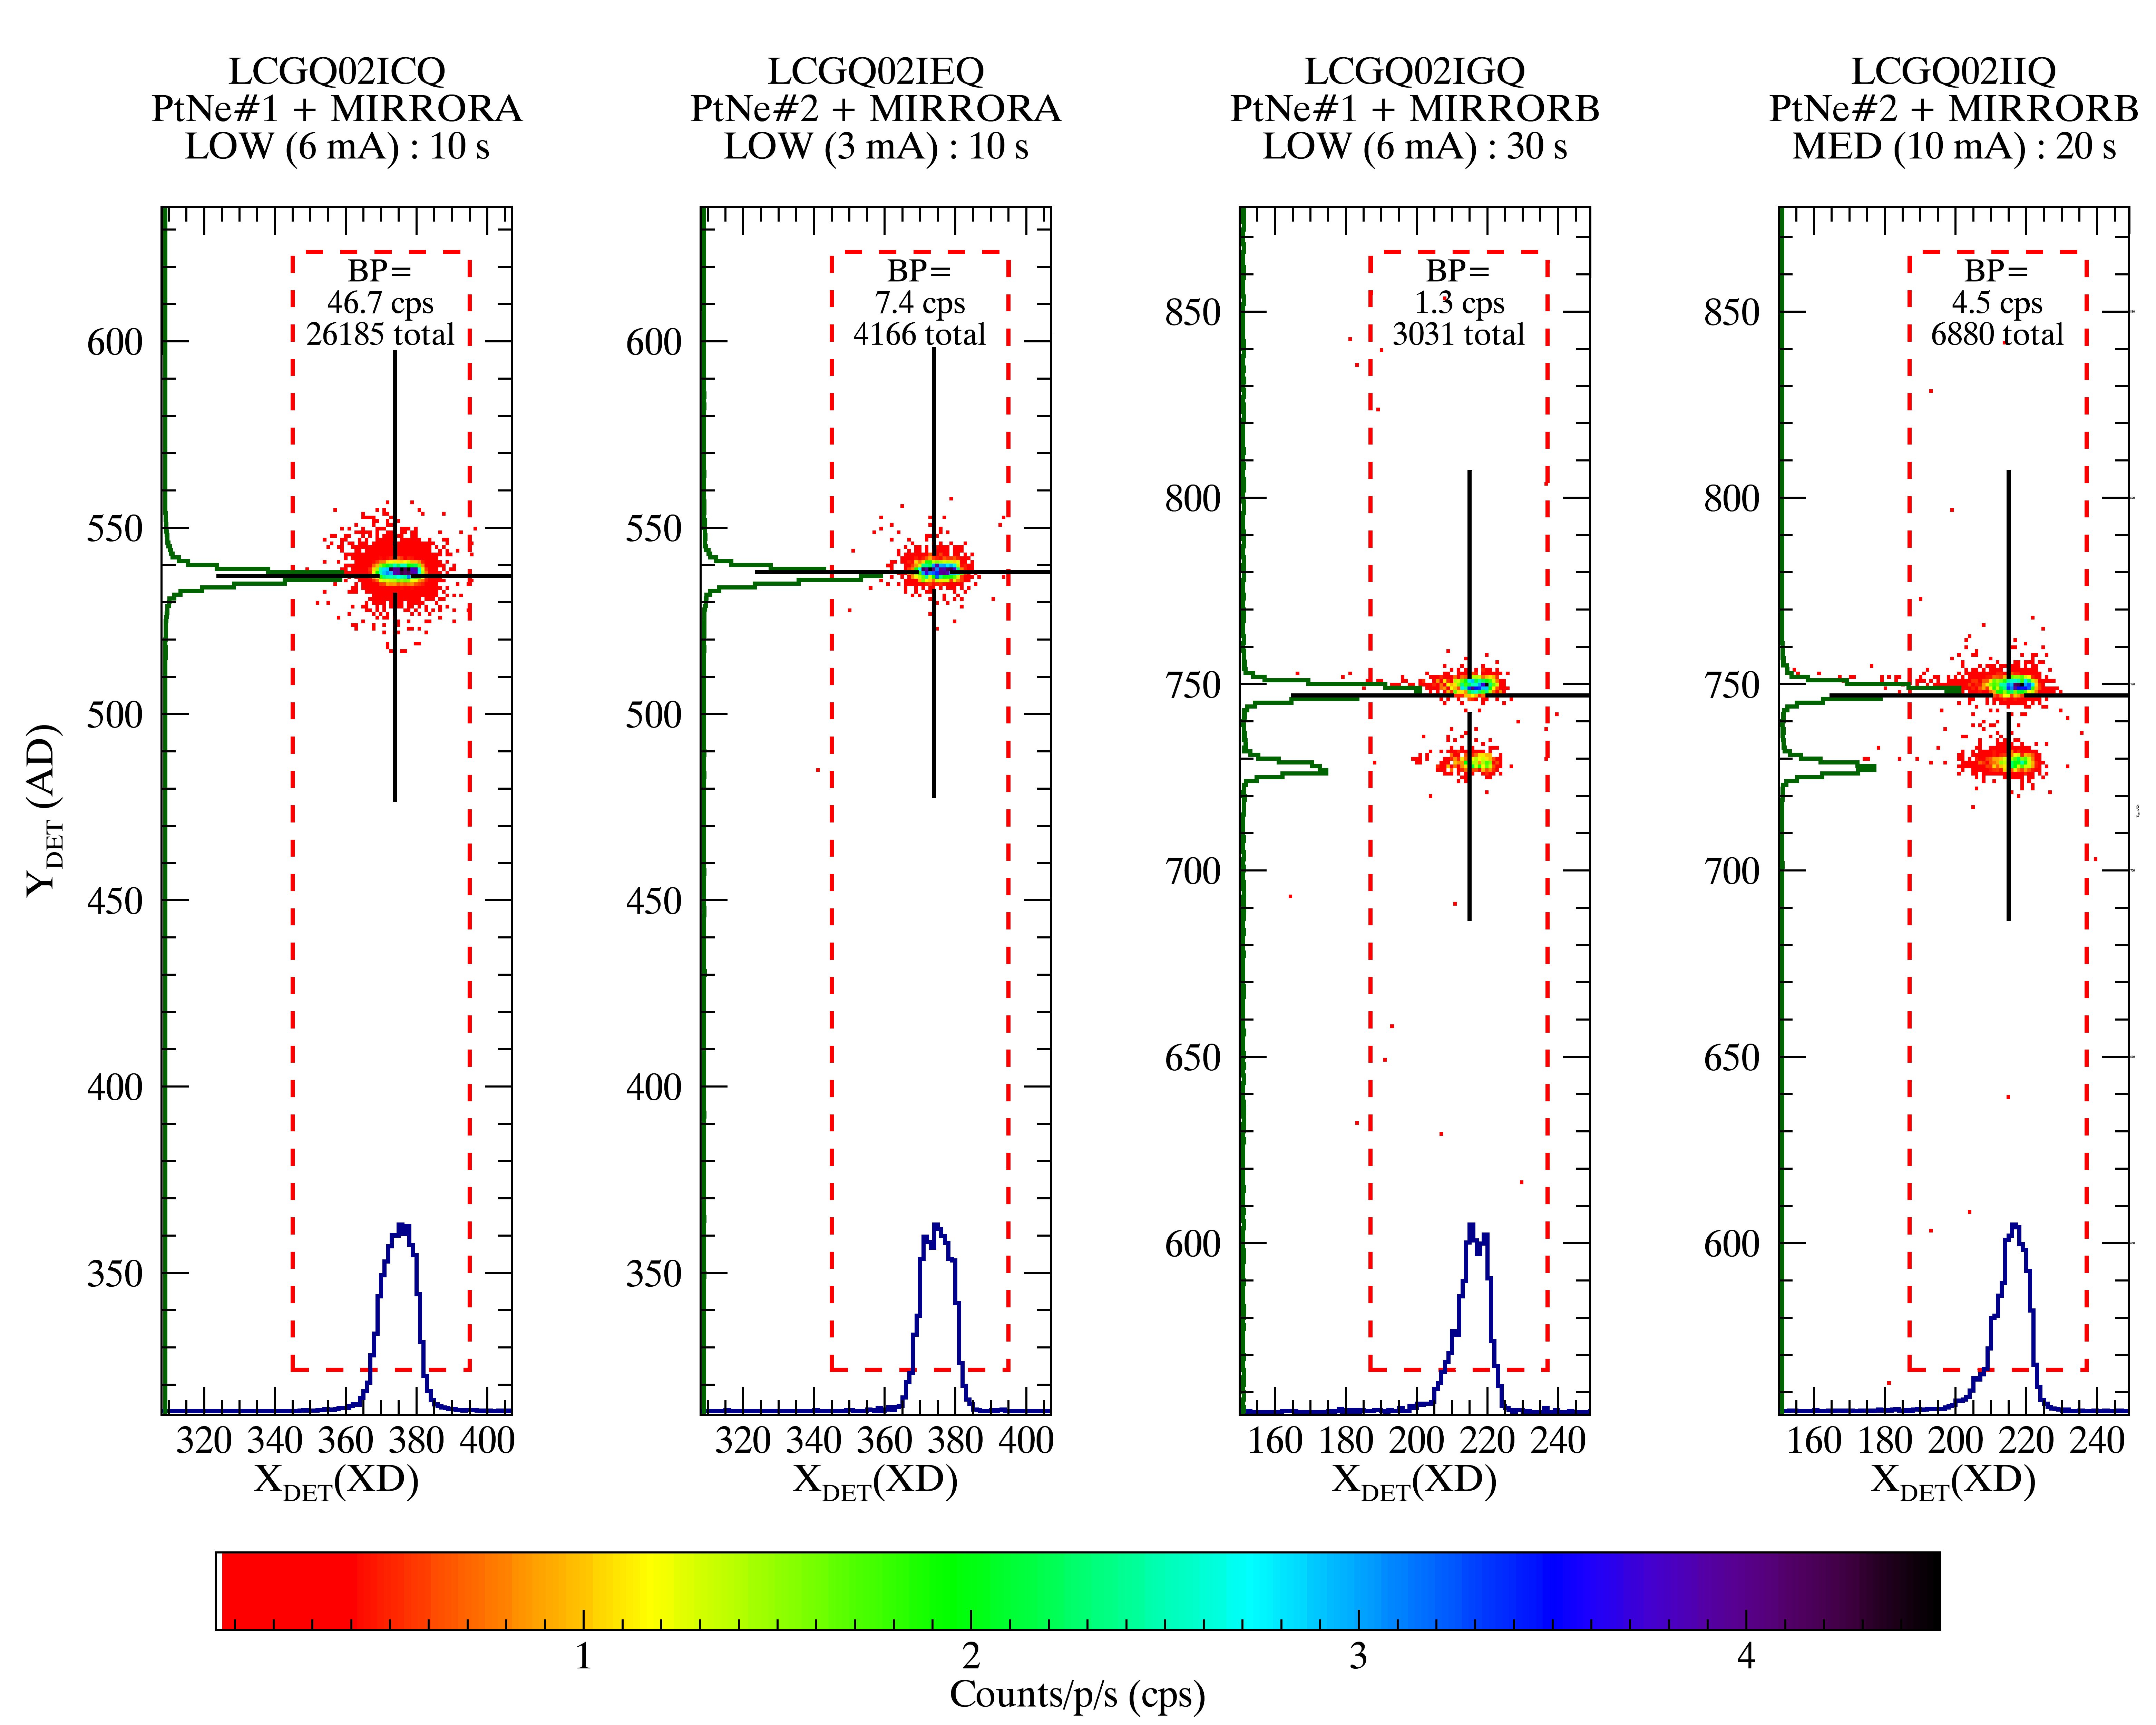
\includegraphics[width=\textwidth]{png/C21_13526_FP.png}
\caption{These four panels show a `family portrait' of the available COS PtNe Lamp + MIRROR combinations possible with \tacq{IMAGE}. Panel titles give the lamp and mirror combination, along with the current setting (in milli-amps, mA) and the exposure times in this program.
These images are in `detector' coordinates, as used on-board COS.
The images show the observed counts/pixel/s (cps) as given by the colorbar on the bottom.
The \textcolor{red}{red} dashed boxes show the Cycle~24 \tacq{IMAGE}~WCA subarrays. At the top of the subarrays, text provides the count rate in the brightest pixel (BP) in units of counts per second per NUV MAMA pixel (cps).
The \textcolor{blue}{blue} histogram on the bottom edge shows the cross-dispersion (XD) lamp profile in detector `X' coordinates, while
the \textcolor{green}{green} histogram on the left edge shows the along-dispersion (AD) lamp profile in detector `Y' coordinates.
The cross-hairs show the median location of the given configurations' lamp events within the TA subarray.
PtNe\#2 lamp was used for all \tacq{IMAGE}s~ during Cycle~24, and was operated at LOW current (6~mA) for those using MIRRORA and MEDium current (10~mA) for those using MIRRORB.
}
\label{fig:FP}
\vspace{1.3cm}
\end{figure}

\begin{figure}[htb]
\noindent\includegraphics*[width=0.795\linewidth]{png/C22_13972_FP.png}
\caption{Cycle~22 PtNe Lamp `Family Portrait'' \ref{fig:FG21}}
\end{figure}

\begin{figure}[htb]
\noindent\includegraphics*[width=0.795\linewidth]{png/C23_14440_FP.png}
\caption{Cycle~23 PtNe Lamp `Family Portrait'' \ref{fig:FG22}}
\end{figure}

\begin{figure}[htb]
\noindent\includegraphics*[width=0.795\linewidth]{png/C24_14857_FP.png}
\caption{Cycle 24 PtNe Lamp `Family Portrait'' \ref{fig:FG21}}
\end{figure}

\begin{figure}[htb]
\noindent\includegraphics*[width=0.795\linewidth]{png/C24_14857_Error_vs_lampSN.png}
\caption{Cycle~24 PtNe Lamp `Family Portrait'' \ref{fig:FG24}}
\end{figure}
\clearpage
\subsection{Verifying the \tacq{PEAKXD} WCA-to-PSA Offsets.} \label{subsec:acqpeakxd}

\tiny
\begin{deluxetable}{lclcccr}
\tablewidth{0pt}
\tabcolsep 10pt
\tablecolumns{7}
\tabletypesize{\footnotesize}
\tablecaption{COS Cycle~24 TA Monitoring Results Summary\label{tab:table_one}}
\tablehead{
\colhead{ACQ} & \colhead{COS} & \colhead{Optical} & \colhead{Direction} & \colhead{Measured Offset\tablenotemark{b}} & \colhead{Requirement} & \colhead{Goal}\\
\colhead{Mode} & \colhead{Channel} & \colhead{Configuration} & \colhead{AD or XD} & \colhead{mas\tablenotemark{a}} & \colhead{mas\tablenotemark{a}} & \colhead{mas\tablenotemark{a}}\\
}
\startdata
\hline
IMAGE	&	NUV	&	PSA+MIRRORA	&	AD	&	20$\pm$14	&	41--105	&	40\\
IMAGE	&	NUV	&	PSA+MIRRORB	&	AD	&	10$\pm$14	&	41--105	&	40\\
IMAGE	&	NUV	&	BOA+MIRRORA	&	AD	&	20$\pm$14	&	41--105	&	40\\
IMAGE	&	NUV	&	BOA+MIRRORB	&	AD	&	15$\pm$14	&	41--105	&	40\\
\hline
IMAGE	&	NUV	&	PSA+MIRRORA	&	XD	&	75$\pm$14	&	300		&	100\\
IMAGE	&	NUV	&	PSA+MIRRORB	&	XD	&	20$\pm$14	&	300		&	100\\
IMAGE	&	NUV	&	BOA+MIRRORA	&	XD	&	95$\pm$14	&	300		&	100\\
IMAGE	&	NUV	&	BOA+MIRRORB	&	XD	&	12$\pm$14	&	300		&	100\\
\hline
PEAKXD	&	NUV	&	G185M		&	XD	&	 70$\pm$17		&	300		&	100\\
PEAKXD	&	NUV	&	G225M		&	XD	&	 60$\pm$17		&	300		&	100\\
PEAKXD	&	NUV	&	G285M		&	XD	&	 20$\pm$17		&	300		&	100\\
PEAKXD	&	NUV	&	G230L		&	XD	&	 20$\pm$17		&	300		&	100\\
PEAKXD	&	FUVA	&	G130M		&	XD	&	-30$\pm$71		&	300		&	100\\
PEAKXD	&	FUVA	&	G160M		&	XD	&	-20$\pm$71		&	300		&	100\\
PEAKXD	&	FUVA	&	G140L		&	XD	&	-170$\pm$71		&	300		&	100\\
\hline
\enddata
\tablenotetext{a}{1 mas = 1 milli-arcsecond.}
\tablenotetext{b}{The quoted error bars are associated with a 0.5 uncertainty when measuring the integer WCA coordinate,
and 1/3 of an NUV pixel when using the \tacq{IMAGE}~checkbox centering algorithm. Added in quadrature, the approximate
\tacq{IMAGE}~measurement error is $\approx 0.6$ NUV pixels, or 14 mas.
Each \tacq{PEAKXD}~ WCA-to-SA measurement contains an error estimate of $\sqrt2 * 0.5 $ times the plate scale of the detector in use
(one half pixel or digital-element uncertainty for each measurement of an integer quantity).
For the NUV channel, this is 23.5 mas/p or $\sqrt2 * 0.5 * 23.5 = 17$ mas.
For the FUV channel, this is $\approx \sqrt2 * 0.5 * 100 \approx 71$ mas.}
\end{deluxetable}

\subsection{New MIRRORB} \label{subsec:newMIRRORB}

\normalsize
\clearpage
\section{Spectroscopic TA Verification}\label{sec:spVER}

After the series of \tacq{IMAGE}s that start each visit, the target should be accurately centered. We take advantage of this to monitor COS spectroscopic TAs.

COS spectroscopic TAs consist of up to three stages \tacq{SEARCH}, \tacq{PEAKD}, and \tacq{PEAKXD}.
The COS spectroscopic \tacq{SEARCH} and \tacq{PEAKD} algorithms do not use any FSW patchable constants, and do not flash the
internal calibration lamps. The only monitoring required for these TA phases is to ensure that the mechanisms were in their proper
positions and that the TA subarrays defined in the HST ground commanding are proper for the mechanism positions used during the acquisitions.

Each FUV central wavelength setting (CENWAVE) uses a unique OSM1 rotation, whereas all NUV TAs use the same OSM1 rotation independent of CENWAVE.
However, each NUV CENWAVE uses a different OSM2 rotation during TA. Each FUV CENWAVE has it's own set of TA subarrays (up to four per segment), while the NUV TA subarrays are not CENWAVE
specific, but are grating specific.

COS TA in the XD direction (\tacq{PEAKXD}) requires the use of XD WCA-to-PSA offsets with the nominal {{\bf NUM$\_$POS}\rm}~=1 algorithm.
These values are contained for both the NUV and FUV channels in the FSW patchable constant table \textsc{pcta\_CalTargetOffset}, and are provided for reference in Table~\ref{tab:wcatopsa}.
All NUV and FUV (LP1, LP2 and LP3) \tacq{PEAKXDs} monitored in this ISR used the original {{\bf NUM$\_$POS}\rm}~=1 algorithm).

The verification process is for \tacq{PEAKXD} is simple, take a normal spectrum with a target signal-to-noise ratio of least 50 for the entire spectrum (2500 target counts) used by \tacq{PEAKXD}.
For NUV exposures, this is the `B' stripe only, and for the FUV, only events on FUVA are used.
TA subarrays are used to mask out any detector hot-spots or Geocoronal light that could interfere with the centering process.

% $Id: pctaWCA2SA.tex,v 1.5 2018/03/30 20:22:12 penton Exp $
\begin{table}
\centering
	\begin{threeparttable}[tbc]
	\caption{\tacq{PEAKXD} WCA-to-PSA offsets}
	\begin{tabular*}{.75\linewidth}{@{\extracolsep{\fill}}lrrr}
		\toprule
		\textit{OPT\_ELEM} &	LP1	&	LP2	&	LP3	\\
		\midrule
		\multicolumn{4}{c}{FUV\tnote{1}}\\
		\midrule
		G130M	&	 -898	&	-943	&	-892 \\
		G140L	&	 -884	&	-950	&	-857 \\
		G160M	&	 -898	&	-933	&	-901 \\
		\midrule
		\multicolumn{4}{c}{NUV\tnote{2}}\\
		\midrule
		G130M	&	 -898	&	-943	&	-892 \\
		G140L	&	 -884	&	-950	&	-857 \\
		G160M	&	 -898	&	-933	&	-901 \\
		\bottomrule
	\end{tabular*}
	\footnotesize
		\begin{tablenotes}
			\item[1] {Divide the FUV numbers by -10 to get the number of XD rows between the PSA and WCA spectra for a target centered in the aperture.}
			\item[2] {Divide the NUV numbers by 10 to get the NUV WCA-to-PSA offset. }
		\end{tablenotes}
	The FSW patchable constant \textsc{pcta\_CalTargetOffsetScale} determines the FSW scaling (currently set to 10).
	FUV scalings are "negative" due to the parity of HST slews relative to the COS coordinate system.
	\label{tab:wcatopsa}
	\normalsize
	\end{threeparttable}
\end{table}

%\begin{deluxetable}{lrrr}
%\tablewidth{0pt}
%\tabcolsep 12 pt
%%\tabletypesize{\footnotesize}
%\tablecolumns{4}
%\tablecaption{\tacq{PEAKXD} WCA-to-PSA offsets \label{tab:wcatopsa}}
%\tablehead{
%\colhead{\textit{OPT\_ELEM}}&\colhead{LP1}&\colhead{LP2}&\colhead{LP3}\\
%}
%\startdata
%\toprule
%\multicolumn{4}{c}{FUV\tablenotemark{f}}\\
%\midrule
%G130M	&	 -898	&	-943	&	-892 \\
%G140L	&	 -884	&	-950	&	-857 \\
%G160M	&	 -898	&	-933	&	-901 \\
%\midrule
%\multicolumn{4}{c}{NUV\tablenotemark{n}}\\
%\midrule
%G185M	&	3742	&	\dots	&	\dots \\
%G225M	&	3746	&	\dots	&	\dots \\
%G230L	&	3734	&	\dots	&	\dots \\
%G285M	&	3749	&	\dots	&	\dots \\
%\bottomrule
%\enddata
%\tablenotetext{f}{Divide the FUV numbers by -10 to get the number of XD rows between the PSA and WCA spectra for a target centered in the aperture.}
%\tablenotetext{n}{Divide the NUV numbers by 10 to get the NUV WCA-to-PSA offset. }
%\tablecomments{The FSW patchable constant \textsc{pcta\_CalTargetOffsetScale} determines the FSW scaling (currently set to 10).
%FUV scalings are "negative" due to the parity of HST slews relative to the COS coordinate system.
%%{\bf Note to reviewers: Do you think I should keep the numbers in their FSW values (not scaled), or should I go ahead and scale them ?}}
%\end{deluxetable}

% $Id: tamon_output.tex,v 1.7 2018/04/16 21:16:03 penton Exp $

\begin{deluxetable}{rrrrrrrrrrrrrrrrrrr}
\tabcolsep 2pt
\tabletypesize{\tiny}
\tablecolumns{19}
\tablecaption{COS TA Monitor \texttt{ACQ/IMAGE} Data}\label{tab:Imagedata}
\tablehead{
\colhead{\textit{ROOTNAME}}&\colhead{\textit{EXPTYPE}}&\colhead{\textit{OPT\_ELEM}}&\colhead{LAMP}&\colhead{Current}&\colhead{Target ET}&\colhead{Lamp ET}&\colhead{WCA}&\colhead{WCA}&\colhead{SA}&\colhead{SA}&\colhead{WtP}&\colhead{WtP}&\colhead{Lamp}&\colhead{Lamp}&\colhead{WCA}&\colhead{Lamp}&\colhead{Lamp}&\colhead{Target}\\
\colhead{}&\colhead{}&\colhead{ }&\colhead{}&\colhead{}&\colhead{(s)}&\colhead{(s)}&\colhead{AD}&\colhead{XD}&\colhead{AD}&\colhead{XD}&\colhead{AD}&\colhead{XD}&\colhead{counts}&\colhead{cps}&\colhead{bck}&\colhead{CPS}&\colhead{BP}&\colhead{BP}\\
\colhead{(1)}&\colhead{(2)} & \colhead{(3)}&\colhead{(4)} &
\colhead{(5)}&\colhead{(6)} & \colhead{(7)}&\colhead{(8)} &
\colhead{(9)}&\colhead{(10)} & \colhead{(11)} &\colhead{(12)} &
\colhead{(13)}&\colhead{(14)} & \colhead{(15)}&\colhead{(16)} &
\colhead{(17)}&\colhead{(18)} & \colhead{(19)}
}
\startdata
\toprule
lcgq01q7q & EXT/SCI & MIRB & P2 & Med &  16 &  16 & 717 & 214 & 763.1 & 588.9 & 46.1 & 374.9 & 4890.0 & 305.6 & 167 & 305.6 & 4.4 & 26.7\\
lcgq01q9q & EXT/SCI & MIRA & P2 & Med & 150 & 150 & 479 & 370 & 550.3 & 739.9 & 71.3 & 369.9 & 1718.0 &\dots&\dots&\dots&\dots& 0.2\\
lcgq01qbq & WAVECAL & MIRA & P2 & Low &   7 &\dots& 503 & 372 & 596.4 & 869.2 & 93.4 & 497.2 & 2964.0 & 423.4 & 61 & 423.4 & 7.7 & 0.3\\
lcgq01qfq & WAVECAL & MIRA & P2 & Low &   7 &\dots& 503 & 372 & 652.2 & 793.2 & 149.2 & 421.2 & 2882.0 & 411.7 & 71 & 411.7 & 7.9 & 0.3\\
lcgq01qhq & EXT/SCI & MIRB & P2 & Med &  12 &  12 & 718 & 212 & 762.9 & 589.3 & 44.9 & 377.3 & 3391.0 & 282.6 & 151 & 282.6 & 3.9 & 19.9\\
lcgq02hoq & WAVECAL & MIRA & P2 & Low &   7 &\dots& 529 & 372 & 891.6 & 635.6 & 362.6 & 263.6 & 2827.0 & 403.9 & 97 & 403.9 & 9.9 & 0.3\\
lcgq02hqq & EXT/SCI & MIRB & P2 & Low & 181 &\dots& 713 & 211 & 784.4 & 582.7 & 71.4 & 371.7 & 2383.0 &\dots&\dots&\dots&\dots& 0.2\\
lcgq02hsq & WAVECAL & MIRB & P2 & Med &  12 &\dots& 738 & 212 & 898.7 & 439.2 & 160.7 & 227.2 & 3683.0 & 306.9 & 165 & 306.9 & 4.8 & 0.2\\
lcgq02hwq & WAVECAL & MIRB & P2 & Med &  12 &\dots& 738 & 213 & 927.8 & 656.8 & 189.8 & 443.8 & 3575.0 & 297.9 & 145 & 297.9 & 3.9 & 0.2\\
lcgq02hyq & WAVECAL & MIRA & P2 & Low &  10 &\dots& 522 & 372 & 451.2 & 711.3 & -70.8 & 339.3 & 4173.0 & 417.3 & 147 & 417.3 & 7.7 & 0.2\\
lcgq02icq & WAVECAL & MIRA & P1 & Low &  10 &\dots& 537 & 374 & 803.3 & 768.3 & 266.3 & 394.3 & 26040.0 & 2604.0 & 120 & 2604.0 & 46.7 & 0.2\\
lcgq02ieq & WAVECAL & MIRA & P2 & Low &  10 &\dots& 538 & 374 & 559.7 & 667.1 & 21.7 & 293.1 & 4036.0 & 403.6 & 122 & 403.6 & 7.4 & 0.2\\
lcgq02igq & WAVECAL & MIRB & P1 & Low &  30 &\dots& 747 & 215 & 879.3 & 654.8 & 132.3 & 439.8 & 2659.0 & 88.6 & 364 & 88.6 & 1.3 & 0.1\\
lcgq02iiq & WAVECAL & MIRB & P2 & Med &  20 &\dots& 747 & 215 & 539.0 & 725.6 & -208.0 & 510.6 & 6620.0 & 331.0 & 250 & 331.0 & 4.5 & 0.1\\
lcri01g1q & EXT/SCI & MIRB & P2 & Med &  12 &  12 & 722 & 210 & 767.7 & 584.2 & 45.7 & 374.2 & 3016.0 & 251.3 & 166 & 251.3 & 4.2 & 30.0\\
lcri01g3q & EXT/SCI & MIRA & P2 & Med & 150 &\dots& 474 & 370 & 552.0 & 735.7 & 78.0 & 365.7 & 1964.0 &\dots&\dots&\dots&\dots& 0.2\\
lcri01g5q & WAVECAL & MIRA & P2 & Low &  10 &\dots& 506 & 372 & 768.5 & 842.0 & 262.5 & 470.0 & 4100.0 & 410.0 & 117 & 410.0 & 9.8 & 0.2\\
lcri01g9q & WAVECAL & MIRA & P2 & Low &  10 &\dots& 506 & 371 & 278.3 & 582.7 & -227.7 & 211.7 & 3960.0 & 396.0 & 148 & 396.0 & 9.2 & 0.2\\
lcri01gcq & EXT/SCI & MIRB & P2 & Med &  14 &  12 & 723 & 212 & 767.4 & 588.9 & 44.4 & 376.9 & 3381.7 & 281.8 & 148 & 281.8 & 4.0 & 28.3\\
lcri02haq & WAVECAL & MIRA & P2 & Low &  14 &\dots& 526 & 372 & 644.1 & 719.4 & 118.1 & 347.4 & 5730.0 & 409.3 & 195 & 409.3 & 8.4 & 0.1\\
lcri02hcq & EXT/SCI & MIRB & P2 & Low & 181 & 181 & 715 & 211 & 782.3 & 578.6 & 67.3 & 367.6 & 2406.0 &\dots&\dots&\dots&\dots& 0.2\\
lcri02heq & WAVECAL & MIRB & P2 & Med &  24 &\dots& 737 & 213 & 853.4 & 647.7 & 116.4 & 434.7 & 7167.0 & 298.6 & 308 & 298.6 & 4.6 & 0.1\\
lcri02hiq & WAVECAL & MIRB & P2 & Med &  24 &\dots& 737 & 213 & 606.7 & 645.2 & -130.3 & 432.2 & 7316.0 & 304.8 & 295 & 304.8 & 4.5 & 0.1\\
lcri02hkq & WAVECAL & MIRA & P2 & Low &  14 &\dots& 519 & 372 & 551.0 & 580.0 & 32.0 & 208.0 & 5840.0 & 417.1 & 203 & 417.1 & 7.9 & 0.1\\
lcri02hyq & WAVECAL & MIRA & P1 & Low &  14 &\dots& 463 & 372 & 683.3 & 807.3 & 220.3 & 435.3 & 36245.0 & 2588.9 & 201 & 2588.9 & 45.5 & 0.1\\
lcri02i0q & WAVECAL & MIRA & P2 & Low &  24 &\dots& 463 & 372 & 781.3 & 778.6 & 318.3 & 406.6 & 9864.0 & 411.0 & 303 & 411.0 & 6.9 & 0.1\\
lcri02i2q & WAVECAL & MIRB & P1 & Low &  30 &\dots& 672 & 213 & 486.2 & 739.8 & -185.8 & 526.8 & 2864.0 & 95.5 & 415 & 95.5 & 1.3 & 0.1\\
lcri02i4q & WAVECAL & MIRB & P2 & Med &  24 &\dots& 671 & 212 & 884.3 & 415.3 & 213.3 & 203.3 & 8082.0 & 336.8 & 312 & 336.8 & 4.9 & 0.1\\
ld3701gvq & EXT/SCI & MIRB & P2 & Med &  16 &  16 & 727 & 210 & 772.8 & 584.3 & 45.8 & 374.3 & 4147.0 & 259.2 & 184 & 259.2 & 4.3 & 19.0\\
ld3701gxq & EXT/SCI & MIRA & P2 & Med & 150 & 150 & 479 & 371 & 551.2 & 735.8 & 72.2 & 364.8 & 1739.0 &\dots&\dots&\dots&\dots& 0.2\\
ld3701gzq & WAVECAL & MIRA & P2 & Low &   9 &\dots& 505 & 372 & 413.8 & 701.7 & -91.2 & 329.7 & 3667.0 & 407.4 & 94 & 407.4 & 8.1 & 0.2\\
ld3701h3q & WAVECAL & MIRA & P2 & Low &  10 &\dots& 505 & 372 & 802.6 & 780.0 & 297.6 & 408.0 & 3999.0 & 399.9 & 107 & 399.9 & 7.6 & 0.2\\
ld3701h5q & EXT/SCI & MIRB & P2 & Med &  16 & 1 6 & 728 & 212 & 773.4 & 589.0 & 45.4 & 377.0 & 4343.0 & 271.4 & 185 & 271.4 & 4.6 & 19.1\\
ld3702n1q & WAVECAL & MIRA & P2 & Low &  14 &\dots& 515 & 371 & 886.6 & 659.4 & 371.6 & 288.4 & 5589.0 & 399.2 & 167 & 399.2 & 7.7 & 0.2\\
ld3702n4q & EXT/SCI & MIRB & P2 & Low & 183 & 183 & 723 & 213 & 774.9 & 577.6 & 51.9 & 364.6 & 2081.0 &\dots&\dots&\dots&\dots& 0.2\\
ld3702n7q & WAVECAL & MIRB & P2 & Med &  24 &\dots& 728 & 212 & 778.9 & 703.3 & 50.9 & 491.3 & 7288.0 & 303.7 & 277 & 303.7 & 4.5 & 0.1\\
ld3702nbq & WAVECAL & MIRB & P2 & Med &  24 &\dots& 728 & 212 & 248.1 & 419.3 & -479.9 & 207.3 & 7140.0 & 297.5 & 274 & 297.5 & 4.5 & 0.1\\
ld3702neq & WAVECAL & MIRA & P2 & Low &  14 &\dots& 507 & 372 & 911.7 & 878.5 & 404.7 & 506.5 & 5622.0 & 401.6 & 153 & 401.6 & 8.1 & 0.1\\
ld3702o1q & WAVECAL & MIRA & P1 & Low &  14 &\dots& 531 & 371 & 485.9 & 883.6 & -45.1 & 512.6 & 37530.0 & 2680.7 & 172 & 2680.7 & 45.6 & 0.1\\
ld3702o3q & WAVECAL & MIRA & P2 & Low &  24 &\dots& 531 & 371 & 665.9 & 888.6 & 134.9 & 517.6 & 9841.0 & 410.0 & 273 & 410.0 & 6.9 & 0.1\\
ld3702o5q & WAVECAL & MIRB & P1 & Low &  30 &\dots& 744 & 211 & 651.6 & 609.1 & -92.4 & 398.1 & 2375.0 & 79.2 & 319 & 79.2 & 1.5 & 0.1\\
ld3702o7q & WAVECAL & MIRB & P2 & Med &  24 &\dots& 743 & 211 & 940.2 & 700.2 & 197.2 & 489.2 & 6674.0 & 278.1 & 283 & 278.1 & 4.2 & 0.1\\
ldozbadjs & EXT/SCI & MIRB & P2 & Med &  16 & 16  & 724 & 210 & 769.8 & 583.4 & 45.8 & 373.4 & 4005.0 & 250.3 & 138 & 250.3 & 4.4 & 20.2\\
ldozbadlq & EXT/SCI & MIRA & P2 & Med &  150& 150 & 472 & 371 & 545.1 & 735.6 & 73.1 & 364.6 & 1462.0 &\dots&\dots&\dots&\dots& 0.2\\
ldozbadnq & WAVECAL & MIRA & P2 & Low &   9 &\dots& 499 & 372 & 889.8 & 583.2 & 390.8 & 211.2 & 3688.0 & 409.8 & 76 & 409.8 & 7.7 & 0.2\\
ldozbadrq & WAVECAL & MIRA & P2 & Low &  10 &\dots& 498 & 372 & 311.8 & 608.8 & -186.2 & 236.8 & 4009.0 & 400.9 & 97 & 400.9 & 7.0 & 0.2\\
ldozbadtq & EXT/SCI & MIRB & P2 & Med &  16 &  16 & 725 & 212 & 769.8 & 588.9 & 44.8 & 376.9 & 4367.0 & 272.9 & 121 & 272.9 & 3.7 & 21.0\\
ldozbblgq & WAVECAL & MIRA & P2 & Low &  14 &\dots& 507 & 372 & 748.6 & 911.9 & 241.6 & 539.9 & 5721.0 & 408.6 & 155 & 408.6 & 8.4 & 0.1\\
ldozbbliq & EXT/SCI & MIRB & P2 & Low &  183&\dots& 713 & 213 & 776.2 & 578.7 & 63.2 & 365.7 & 2283.0 &\dots&\dots&\dots&\dots& 0.2\\
ldozbblkq & WAVECAL & MIRB & P2 & Med &  24 &\dots& 730 & 212 & 585.6 & 716.8 & -144.4 & 504.8 & 6957.0 & 289.9 & 331 & 289.9 & 4.7 & 0.1\\
ldozbbloq & WAVECAL & MIRB & P2 & Med &  24 &\dots& 730 & 212 & 703.1 & 689.2 & -26.9 & 477.2 & 6983.0 & 291.0 & 305 & 291.0 & 4.0 & 0.1\\
ldozbblqq & WAVECAL & MIRA & P2 & Low &  14 &\dots& 510 & 372 & 380.6 & 845.9 & -129.4 & 473.9 & 5566.0 & 397.6 & 177 & 397.6 & 7.9 & 0.1\\
ldozbbm4q & WAVECAL & MIRA & P1 & Low &  16 &\dots& 503 & 371 & 815.0 & 659.6 & 312.0 & 288.6 & 42548.0 & 2659.2 & 189 & 2659.2 & 44.2 & 0.1\\
ldozbbm6q & WAVECAL & MIRA & P2 & Low &  26 &\dots& 503 & 371 & 772.1 & 616.6 & 269.1 & 245.6 & 10476.0 & 402.9 & 300 & 402.9 & 7.6 & 0.1\\
ldozbbm8q & WAVECAL & MIRB & P1 & Low &  32 &\dots& 715 & 211 & 252.8 & 463.5 & -462.2 & 252.5 & 2714.0 & 84.8 & 407 & 84.8 & 1.4 & 0.1\\
ldozbbmaq & WAVECAL & MIRB & P2 & Med &  26 &\dots& 715 & 211 & 560.5 & 575.1 & -154.5 & 364.1 & 7768.0 & 298.8 & 340 & 298.8 & 3.7 & 0.1\\
ldozpbf7q & EXT/SCI & MIRA & P2 & Low &  20 &  20 & 511 & 370 & 555.5 & 741.6 & 44.5 & 371.6 & 7790.0 & 389.5 & 269 & 389.5 & 7.3 & 17.2\\
ldozpbf9q & EXT/SCI & MIRB & P2 & Med & 220 &  40 & 734 & 210 & 779.2 & 582.8 & 45.2 & 372.8 & 12877.2 & 321.9 & 523 & 321.9 & 3.5 & 0.6\\
ldozpbfdq & EXT/SCI & MIRB & P2 & Med & 220 &  40 & 734 & 211 & 780.3 & 584.0 & 46.3 & 373.0 & 13043.9 & 326.1 & 505 & 326.1 & 3.5 & 0.8\\
ldozpbffq & EXT/SCI & MIRA & P2 & Low &  20 &  20 & 514 & 370 & 559.3 & 743.2 & 45.3 & 373.2 & 7798.0 & 389.9 & 285 & 389.9 & 7.1 & 23.4\\
\enddata
\tablecomments{{\bf Note to reviewer: Some of the numbers in this table are odd, I am researching.}}
\end{deluxetable}

\subsection{NUV Spectroscopic TA verification}\label{subsec:NspVER}
\subsection{FUV Spectroscopic TA verification}\label{subsec:FspVER}

%\begin{deluxetable}{|r|r|r|r|r|r|r|r|r|r|r|}
\tabcolsep 10pt
\tabletypesize{\footnotesize}
\tablecolumns{11}
%\tablewidth{0 pt}
\tablecaption{ACQ/PEAKXD Verification: WCA-to-PSA offsets\label{table:peakxd}}
\tablehead{\colhead{IPPPSSOOT}&
\colhead{Grating}&\colhead{Cenwave\tablenotemark{a}}&\colhead{Exptime\tablenotemark{b}}&
\colhead{SN^\tablenotemark{c}} &
\colhead{WCA\tablenotemark{d}}&\colhead{PSA\tablenotemark{e}} &
\colhead{WtP\tablenotemark{f}}&\colhead{eWtP\tablenotemark{g}} &
\colhead{Offset\tablenotemark{h}}&\colhead{Offset\tablenotemark{i}} \\

\colhead{}&\colhead{}&\colhead{(\AA)}&\colhead{(sec)}&
\colhead{}&\colhead{(XD)}&\colhead{(XD)} &
\colhead{(rows)}&\colhead{(rows)} &
\colhead{(rows)}&\colhead{(\arcsec)}
}
\startdata
\hline \multicolumn{11}{|c|}{Cycle~21 (P14440)}\\ \hline
\hline \multicolumn{11}{|c|}{Cycle~22 (P14440)}\\ \hline
\hline \multicolumn{11}{|c|}{Cycle~23 (P14440)}\\ \hline
\hline \multicolumn{11}{|c|}{Cycle~24 (P14440)}\\ \hline
\multicolumn{11}{|c|}{Visit 01 : Target = WD1657+343}\\
\hline
lcri01ggq & G230L & 3000 &  20&  55 & 374.00 & 747.00 & 373.00 & 373.40 &  -0.40 &  -0.01\\
lcri01giq & G285M & 2676 & 151&  94 & 351.00 & 726.00 & 375.00 & 374.90 &  0.10 &  0.00\\
lcri01gkq & G130M & 1309 &  20& 175 & 537.32 & 448.98 & -88.34 & -89.20 &  0.86 &  -0.08\\
lcri01h6q & G140L & 1280 &  7&  82 & 544.55 & 457.36 & -87.20 & -85.70 &  -1.50 &  -0.15\\
\hline
\multicolumn{11}{|c|}{Visit 02 : Target = HIP6657}\\
\hline
lcri02hoq&G225M&2306&  52& 178& 371.00& 747.00& 376.00& 374.60&  1.40&  0.03 \\
lcri02hqq&G185M&1913&  40& 205& 367.00& 742.00& 375.00& 374.20&  0.80&  0.02 \\
lcri02hsq&G160M&1600&  22& 281& 531.78& 442.13& -89.65& -90.10&  0.45&  -0.04 \\
lcri02huq&G160M&1600&  25& 272& 531.48& 449.64& -81.84& -90.10&  8.26&  -0.75 \\
lcri02hwq&G160M&1600&  25& 278& 531.73& 434.22& -97.51& -90.10&  -7.41&  0.67 \\
\hline
\enddata

\tablenotetext{a}{Central wavelength setting.}
\tablenotetext{b}{Exposure time in seconds.}
\tablenotetext{c}{Total Signal-to-Noise in Target sqectrum ($\sqrt\rm(Target Counts)}$.}
\tablenotetext{d}{XD centroid of the WCA spectrum. For NUV spectra, this is the median wavelength calibration
lamp photon 'Y'. For FUV spectra, this is mean 'Y' lamp photon location.}
\tablenotetext{e}{XD centroid of the target spectrum taken through the PSA. For NUV spectra, this is the median target photon 'Y'.
For FUV spectra, this is mean 'Y' target photon location.}
\tablenotetext{f}{The difference in the Y locations of the measured WCA and PSA spectra (PSA - WCA).}
\tablenotetext{g}{The expected (PSA-WCA) value. This is the value in the FSW used by ACQ/PEAKXD to center the target in the XD.}
\tablenotetext{h}{Offset of (PSA-WCA) from a perfectly centered measured in 'Y' rows.}
\tablenotetext{i}{Offset of (PSA-WCA) in arcseconds (\arcsec). Note that the platescales are different for each grating and LP. Our goal is to always center the target in the XD to within 0.3\arcsec, with
the 1$\sigma$ goal of 0.1\arcsec.}
\end{deluxetable}


\section{Results}\label{sec:results}
The main results of the HST Cycle~21--24 COS TA monitoring program are as follows:
\begin{description}
\item{\bf SIAF:}{
	All COS NUV \tacq{IMAGE}s~use identical SIAF entries ({\it LFPSA} or {\it LFBOA}).
	Previously, the exposures in the Cycle~23 FGS-to-SI Alignment program (14452) gave a good estimate of the accuracy of the existing NUV LP1 {\it LFPSA}/{\it LFBOA} SIAF entries
	as P14452 performed a PSA/MIRRORA \tacq{IMAGE} on a target whose position was already determined by cross-calibration of the other HST Science Instruments (SI).
	For Cycle~23, data from P14452 indicated that the NUV SIAF entry was accurate to at least [AD,XD] = [0.02,0.08]$\arcsec$.\footnote{As determined from the initial pointing before the first COS \tacq{IMAGE}~of the program.}
	No SIAF adjustments were identified as being needed for NUV (LP1) or FUV (LP3) from this program.\footnote{Long term SIAF monitoring is used to track any mechanical drift in the location of the COS aperture mechanism or any changes to the FGS-to-SI alignment that will need adjusting.
	The last such adjustment was in Cycle~22 (February 2, 2014), while COS FUV observations were at LP2. At this time, all COS entries (NUV and FUV) were adjusted in [V2,V3] by [0.077, -0.070]". }

}
\item{\bf TA Subarrays:} Visual inspection of NUV images, and a review of the photon lists of the NUV and FUV spectra, indicate that all TA subarrays are appropriately defined for Cycle~24 and no adjustments were necessary.
\item{\bf NUV Imaging TAs:}
	The COS \tacq{IMAGE}~ tests in P14452 indicate that the centering achieved with a PSA/MIRRORB \tacq{IMAGE}~is co-aligned with a PSA/MIRRORA \tacq{IMAGE}~to within [AD,XD] $\approx [0.010,0.020]\arcsec$, with a measurement error of approximately $0.014\arcsec$.
	\tacq{IMAGE}~ tests in P14857 reveal that BOA/MIRRORA is co-aligned with PSA/MIRRORB to within [AD,XD] $\approx [0.015,0.100]\arcsec$,
	\footnote{The larger XD alignment error is due to a frequent 1 aperture XD (XAPER) step mechanism position error (1 step ~ $0.048\arcsec$).}
	and that BOA/MIRRORB is co-aligned with BOA/MIRRORA to within [AD,XD] $\approx [0.007,0.062]\arcsec$.

	As shown in Figure~\ref{fig:FP}, P14587 obtained a `family portrait' of Cycle~24 wavelength calibration aperture (WCA) lamp images. These images of PtNe lamp light seen through the WCA
	are used during the LTAIMCAL portion of the LTAIMAGE (ACQ/IMAGE) TA FSW routine to locate the position of the aperture mechanism before centering the target.
	While COS TAs have used the PtNe\#2 lamp for all TAs since installation, images of both lamps (PtNe\#1 and PtNe\#2) are taken annually with both MIRRORs
	(MIRRORA and MIRRORB) to monitor the observed count rates. No changes were observed in the PtNe lamp count rates between Cycles~23 and 24.
	\clearpage
\item{\bf NUV Spectroscopic TAs:}
	The G285M and G230L WCA-to-PSA offsets were measured after a PSA/MIRRORB \tacq{IMAGE}, and were within a XD offset of $0.020\arcsec$ of the FSW value for each grating.
	\footnote{Spectroscopic NUV WCA-to-PSA offsets are determined using a median photon lamp and/or target XD position in the appropriate subarray. The difference between the positions is compared to the FSW value, accounting for any measured offset in the preceding \tacq{IMAGE}.}
	The G185M and G225M offsets were measured after a BOA/MIRRORA \tacq{IMAGE}, and were measured to be within a XD offset of $0.070\arcsec$ and $0.060\arcsec$, respectively, of the FSW value.
	Spectroscopic TAs for all NUV gratings met both the $0.3\arcsec$ requirement and the $0.1\arcsec$ goal.
\item{\bf FUV Spectroscopic TAs:}
	The G130M and G140L WCA-to-PSA offsets were measured after the same PSA/MIRRORB \tacq{IMAGE}~as the G285M and G230L observations.
	The measured offsets were determined to be offset from the FSW values by $\approx -0.030\arcsec$ and $-0.170\arcsec$, respectively, with a measurement error estimated at $0.070\arcsec$.
	The G160M offset was measured after the BOA/MIRRORA \tacq{IMAGE}~used for the G185M and G225M observations. The G160M offset was determined to have a WCA-to-PSA XD offset of $-0.020 \pm 0.070\arcsec$ of the FSW WCA-to-PSA value.
footnote{Spectroscopic FUV WCA-to-PSA offsets are determined using a mean photon lamp and/or target XD position in the appropriate subarray. The difference between the positions is compared to the FSW value, accounting for any measured offset in the preceding \tacq{IMAGE}.}
	Spectroscopic TAs for all FUV gratings met the $0.3\arcsec$ requirement and the G130M and G160M gratings achieved the $0.1\arcsec$ goal.

\end{description}
\vspace{-0.3cm}
\section{Conclusions.\label{theend} }
\vspace{-0.3cm}
	It's all good.

\clearpage
%%%%%%%%
%Acknowledgements
%%%%%%%%
\vspace{-0.3cm}
\section*{Acknowledgements}
\vspace{-0.3cm}
%%%%%%%%
%Change History
%%%%%%%%
\vspace{0.3cm}
%Put instrument, year, and ISR number
\section*{Change History for COS ISR 2018-XX}\label{sec:History}
\vspace{0.3cm}
%Put publication date
Version 1: 30-March-2018 Original Draft Document
%%%%%%%%
%References
%%%%%%%%
\vspace{0.3cm}
\section*{References}\label{sec:References}
\vspace{0.3cm}

\noindent ()
Penton, S., 2016, COS Instrument Science Report 2019-09\\
Cycle~22 IHB\\
Cycle~23 IHB\\
Cycle~24 IHB\\
TAACOS1\\
TAACOS2\\
Keyes, T., \& Penton, S. COS 2010-14 (v1) (HST+COS Target Acquisition Guidelines, Recommendations, and Interpretation)\\
Penton, S. 2011, COS TIR 2010-03 (On-Orbit Target Acquisitions with HST+COS)\\
Roman-Duval, J, 2015, COS ISR2015-02 (Summary of the COS Cycle 20 Calibration Program: P13124)\\
Sana, H., et. al., 2015, COS ISR 2015-06 (Summary of the COS Cycle 21 Calibration Program: P13526))\\
Sonnetrucker, P., et. al., 2016, COS ISR 2016-03 (Summary of the COS Cycle 22 Calibration Program : P13972) \\
Penton, S. 2016, COS ISR 2016-09 (Cycle~22 HST+COS Target Acquisition Monitoring Summary (P13972)\\
Penton, S. 2017, COS ISR 2017-18 (Cycle~23 HST+COS Target Acquisition Monitoring Summary (P14440)\\
Penton, S. \& White, J. 2018, COS ISR 2018-{\bf XX} (Cycle~24 HST+COS Target Acquisition Monitoring Summary (P14857)\\
\newpage
%%%%%%%%
%Appendix
%%%%%%%%
\vspace{-0.3cm}
\section*{Appendix A}\label{sec:Appendix}
\vspace{-0.3cm}
\end{document}
